%\documentclass[b5paper,twoside,10pt,sabonnumbers]{RJWThesis}
\documentclass[a4paper,oneside,12pt,sabonnumbers]{RJWThesis}

\usepackage{amsthm}
\usepackage{amssymb}
\usepackage{eucal}
\usepackage{euler}
\usepackage[plain,chapter]{algorithm}
\usepackage{algorithmic}
\usepackage{listings}

\lstset{
  basicstyle=\footnotesize\sf,
  keywordstyle=\bfseries,
  commentstyle=\footnotesize\itshape,
  stringstyle=\ttfamily,
  flexiblecolumns=true,
  numbers=left,
  numberstyle=\tiny,
}

% \includeonly{fractals/fractals}

%% Use scalable, PostScript Type 1 versions of the Computer Modern fonts.
\usepackage{type1cm}

%% Replace the standard Computer Modern Typewriter font LaTeX uses
%% for monospace text with the PostScript font Adobe Courier.
\usepackage{courier}

% To print crop marks
%\usepackage[a4,cam,center]{crop}
%\crop[font=\upshape\mdseries\small\textsf]

\bibliographystyle{abbrv}

\usepackage[pdfborder=0 0 0,draft=false]{hyperref}
\usepackage{graphicx}
\usepackage{pslatex}
\usepackage{palatino}
%% If you have Sabon, uncomment this
%% \usepackage{sabon}
\usepackage{stmaryrd}
\usepackage{amsmath}
\usepackage{amssymb}
\usepackage{url}

% Global macros used throughout thesis

\newtheorem{thm}{Theorem}
\newtheorem{lemma}{Lemma}
\newtheorem{definition}{Definition}
\newtheorem{cor}{Corollary}
\newtheorem{alg}{Algorithm}
\newenvironment{proof}[1][Proof]{\begin{trivlist}
\item[\hskip \labelsep {\bfseries #1}]}{\qed\end{trivlist}}
\newcommand{\dt}{\cdot}
\newcommand{\nn}{\nonumber}
\newcommand{\half}{\frac{1}{2}}
\newcommand{\magof}[1]{\left\Vert #1 \right\Vert}
\newcommand{\sinc}{\mathrm{sinc}}
\newcommand{\sinhc}{\mathrm{sinhc}}
\newcommand{\cperp}{c_\perp}
\newcommand{\cpar}{c_\parallel}
\newcommand{\rinterp}{\mathrm{rinterp}}
\newcommand{\linterp}{\mathrm{linterp}}
\newcommand{\qinterp}{\mathrm{qinterp}}
\newcommand{\interp}{\mathrm{interp}}
\newcommand{\slerp}{\mathrm{slerp}}
\newcommand{\qed}{\hfill$\boxempty$}
\newcommand{\libcga}{{\tt libcga}}
\newcommand{\libcgadraw}{{\tt libcgadraw}}
\newcommand{\cala}{\mathcal{A}}

\newcommand{\hugewedge}{\bigwedge}

\newcommand{\Jperp}{{J_\perp}}
\newcommand{\Jpar}{{J_\parallel}}
\newcommand{\Jparperp}{{J_{\perp\parallel}}}

\begin{document}

\begin{frontmatter}
\renewcommand{\baselinestretch}{1.2}\selectfont
\title{Computer Graphics using Conformal Geometric Algebra}
\subtitle{A dissertation submitted to the\\{\sc University of 
    Cambridge}\\for the degree of\\{\sc Doctor of Philosophy}}
\author{Richard James Wareham\thanks{Robinson College}}
\group{Signal Processing and Communications Laboratory}
\department{Department of Engineering}
\maketitle
\cleardoublepage

% Front matter
\vspace*{0.2\textheight}
\noindent Copyright \copyright \number\year\ Richard James Wareham.
\vspace*{1em}\\
% \noindent Draft version.\\
\noindent This thesis contains no more than \input{wordcount.txt} words.
\vfill
\noindent Typeset using the \LaTeX{} document preparation system
in the Sabon, Georgia and Computer Modern fonts.
\vfill
\noindent {\sc Signal Processing and Communications Laboratory,}\newline
Department of Engineering,\newline
University of Cambridge,\newline
Trumpington Street,\newline
Cambridge, CB2 1PZ, U.K.
\cleardoublepage

\dedication{To my parents and\\ all those that helped\\ me get here}

\tableofcontents
\listoffigures
\listoftables
\end{frontmatter}

\begin{mainmatter}
\renewcommand{\baselinestretch}{1.75}\selectfont
\begin{savequote}
\quoteperson{You know we all became mathematicians for the same reason: 
  we were lazy.}{Max Rosenlicht}
\end{savequote}

\chapter{Introduction}

It has long been known that going to a four-dimensional, projective, description
of three-dimensional Euclidean geometry can have various advantages --- particularly
when intersections of planes and lines are required. Such
projective descriptions are used extensively in computer vision
where rotations and translations can be described by a single
$4\times 4$ matrix and non-linear projective transformations
become linear. 
Since its inception in the mid-1970s, Computer Graphics (CG) has almost
universally used linear vector algebra as its mathematical framework.
This is due primarily to two factors; most early practitioners of
computer graphics were mathematicians familiar with it and 
linear algebra provided a compact, efficient way of representing points, 
transformations, lines, etc.

In the early-1980s CG moved out of the realm of Computer
Science research and started to be used in the broader scientific 
community as an important research tool, both for simulation and visualisation.
Computer Graphics was still tied to classical vector algebra which
had started to show a number of problems when applied to the problems
being investigated. Amongst these were poor generalisation to
spaces other than $\mathbb{R}^3$ and great conceptual difficulty 
in extending problems to non-Euclidean spaces and
manipulating geometric objects other than simple lines, planes and points.

As computing power becomes cheaper, the opportunity
arises to investigate new
frameworks for CG which, although not providing the time/space
efficiency of vector algebra, may provide a conceptually simpler
system or one of greater analytical power. This thesis presents 
Geometric Algebra (GA) as one such approach.
As one might hope the original four-dimensional description of projective geometry fits
very nicely into the Geometric Algebra framework\cite{HZ91,IJPR00}. 

\section{A Brief Overview of Geometric Algebra}

As stated above, classical vector algebra has a number of problems
once one moves away from three-dimensional Euclidean space. Perhaps the
clearest example is the cross-product of two vectors; the product, $\mathbf{a}
\times \mathbf{b}$, is conventionally defined as a vector normal to the plane
that $\mathbf{a}$ and $\mathbf{b}$ both lie in and has magnitude $ab\sin\theta$
where $\theta$ is the angle between $\mathbf{a}$ and $\mathbf{b}$. However, the
normal to the plane is only uniquely defined in three-dimensions and has no meaning
in 2- or 1-dimensional space; the cross-product does not generalise to
higher-dimension spaces. The product is an important element of vector
algebra and one can see that performing geometric operations in higher-spaces
without it quickly becomes complex.

\subsection{The products}

It was in an attempt \cite{GA:grassmann} to create an algebra of vectors which 
did generalise
to higher spaces that a German schoolteacher named Hermann 
Gra{\ss}mann (1809--1877) created an \emph{exterior} 
or \emph{outer} product of two
vectors denoted as $a \wedge b$. 
%Note that we have dropped the normal
%typographic convention of denoting vectors in boldface for
%reasons which will become clear later.

Gra{\ss}mann's outer product can be visualised geometrically as moving
one vector along the other to form a `directed area'. This is a new object,
neither a vector or a scalar. We shall refer to it as a \emph{bivector}.
Similarly one may form the outer product of this bivector with another
vector to form a directed volume or \emph{trivector}. We say a 
bivector has grade 2, a trivector has grade 3 and, generally, a
$n$-vector has grade $n$.

\begin{figure}
\centering
\includegraphics{geometric}
\caption{Illustration of bi- and trivectors\label{fig:geometric}}
\end{figure}

The geometric objects are illustrated in figure \ref{fig:geometric}. A 
key feature is that the outer-product is anti-commutative and 
associative so that
\begin{displaymath}
a \wedge b = - ( b \wedge a)\quad\mbox{and}\quad 
a \wedge (b \wedge c) = (a \wedge b) \wedge c = a \wedge b \wedge c
\end{displaymath}

Most of Gra{\ss}mann's work was largely ignored by the mathematical community.
It was not until William Clifford (1845--1879) investigated Gra{\ss}mann's
algebra in 1878 \cite{GA:clifford} that the crucial step was made.

Clifford unified Gra{\ss}mann's outer product and the familiar dot
or inner-product into one geometric product such that
\begin{displaymath}
ab = a\cdot b + a \wedge b
\end{displaymath}

A second glance at this shows an interesting feature which should be noted.
In the expression above we are adding a scalar ($a \cdot b$) to a 
bivector ($a \wedge b$). This combination of different objects is
analogous to complex numbers where we linearly combine
a real and imaginary number to form a complex number. In this case we
refer to a linear combination of objects of varying grade as a
\emph{multivector}. Since the algebra may be extended to deal with
multivectors we no longer need different notation for scalars, vectors,
bivectors, etc. This project will use the convention of using lower-case
letters to refer to single-grade objects and upper-case letters to refer
to multivectors. The geometric product also gives us a convenient new
definition of the outer and inner products for vectors
\[
A \wedge B = \frac{1}{2}(AB - BA)
\]
\[
A \cdot B = \frac{1}{2}(AB + BA)
\]

The power of this approach may be illustrated through its application
to rotation. In two dimensions this is easily performed using complex numbers. Representing
the vector $[x\ y]$ as the complex number $z = x + iy$, rotation by
$\theta$ radians can be performed by multiplication with $e^{i\theta}$.
William Hamilton (1805--1865) worked for many years to extend this approach
to three-dimensions. He eventually created \emph{quaternions} \cite{hamilton2,hamilton1},
an algebra with 4 
elements $\left\{1, \mathbf{i}, \mathbf{j}, \mathbf{k}\right\}$ which, although
functional, lacked an obvious geometrical interpretation and again didn't
generalise easily to higher-dimensions.

\subsection{Rotation via Rotors}

To demonstrate Clifford's approach, consider three orthonormal basis
vectors of $\mathbb{R}^3$, $\left\{e_1, e_2, e_3\right\}$. We can form
3 different bivectors from these vectors:
\begin{displaymath}
B_1 = e_2e_3,\quad B_2 = e_3e_1,\quad B_3 = e_1e_2
\end{displaymath}

Note that these are indeed bivectors since
\[
e_ie_j = e_i \cdot e_j + e_i \wedge e_j = e_i \wedge e_j \quad \mbox{iff} \quad i \ne j
\]

Now consider the effect of $B_3$ on the vectors $e_1$ and $e_1 + e_2$:
\begin{displaymath}
e_1B_3 = e_1e_1e_2 = e_1^2e_2=e_2 
\end{displaymath}
\begin{displaymath}
(e_1 + e_2)B_3 = e_1B_3 + e_2B_3 = e_2 + e_2e_1e_2 = e_2 - e_1e_2^2 = e_2 - e_1
\end{displaymath}

\begin{figure}
\centering
\includegraphics{rotation}
\caption{The rotation effect of bivector $B_3 = e_1e_2$\label{fig:rotation}}
\end{figure}

By looking at figure \ref{fig:rotation} it is clear that $B_3$ has the
effect of rotating the vectors counter-clockwise by 90 degrees. It is, in
fact, a general property that the bivector $e_ie_j$ will rotate a
vector 90 degrees in the plane defined by $e_i$ and $e_j$. At first 
glance this seems to offer little more than quaternions but at no point 
have we assumed that we are working in three-dimensional space; this method
also works in higher-dimension spaces.

Now we extend to general rotations. Firstly it is trivial to
show that $B_3$ squares to $-1$:
\begin{displaymath}
B_3^2 = e_1e_2e_1e_2 = -e_1e_2e_2e_1 = -1
\end{displaymath}

We can represent any vector $Z$ in the plane defined by $e_1$ and
$e_2$ using
\begin{eqnarray*}
Z & = & r ( e_1 \cos \theta + e_2 \sin \theta) \\
  & = & e_1 r ( \cos \theta + B_3 \sin \theta)
\end{eqnarray*}
where $r$ is the distance of the point $Z$ from the origin
and $\theta$ is the angle $Z$ makes to $e_1$. Also note
that $e_1B_3 = e_1^2e_2 = e_2$. By taking the Taylor expansion of cosine
and sine and re-arranging the coefficients it can be shown that
\[
e^{B_3\theta} = \cos \theta + B_3 \sin \theta
\]
which is the analogous form of de Moivre's theorem for complex
numbers.

We can thus represent any vector $Z$ which lies in the plane of the
bivector $B_3$ by
\[
Z=e_1re^{B_3\theta}
\]

From this the same argument used for rotation in the complex plane 
can be used to show that rotation by
$\phi$ radians in the plane of $B_3$ is accomplished by $Z \mapsto Z'$
where
\begin{displaymath}
Z' = Ze^{B_3\phi} = Z (\cos \phi + B_3 \sin \phi)
\end{displaymath}

This has all taken place in two dimensions for the moment but note that nothing
in our development has assumed this. In fact we can define a bivector $B_3 = ab$ in
three dimensions and rotate vectors in the place defined by $a$ and $b$ using
the expression above.

\begin{figure}
\centering
\includegraphics{rotation2}
\caption{Rotating vectors in arbitrary planes\label{fig:rotation2}}
\end{figure}

Careful consideration must be given to the case where the vector to be
rotated, $x$, does not lie on the plane of rotation as in figure
\ref{fig:rotation2}. Firstly decompose the
vector into a component which lies in the plane $x_\parallel$ and one
normal to the plane $x_\perp$
\[
x = x_\parallel + x_\perp
\]

Now consider the effect of the following
\begin{eqnarray*}
e^{-B_3\phi/2}
x
e^{B_3\phi/2}
& = & \left(\cos \frac{\phi}{2} - B_3 \sin \frac{\phi}{2}\right)
(x_\parallel + x_\perp )
\left(\cos \frac{\phi}{2} + B_3 \sin \frac{\phi}{2}\right) \\
& = & x_\parallel (\cos \phi + B_3 \sin \phi) + x_\perp\\ 
\end{eqnarray*}
since bivectors anti-commute with vectors in their plane (e.g. 
$e_1(e_2e_1) = -e_2 = -(e_2e_1)e_1$) and commute with
vectors normal to the plane (e.g.\ $e_1(e_2e_3) = (e_2e_3)e_1$).
We have thus succeeded in rotating the component of the vector 
which lies in the plane without affecting the component normal
to the plane --- we have rotated the vector around an axis normal to
the plane.

%and hence
%\begin{eqnarray*}
%Z (\cos \phi + B_3 \sin \phi) & = & (\cos \phi - B_3 \sin \phi)Z \\
%& = &
%\left(\cos \frac{\phi}{2} - B_3 \sin \frac{\phi}{2}\right)
%Z
%\left(\cos \frac{\phi}{2} + B_3 \sin \frac{\phi}{2}\right)
%\end{eqnarray*}

This leads to a general method of rotation in any plane; we
form a bivector of the form $R = \exp({-B\phi/2})$ for a given rotation 
$\phi$ in a plane specified by the bivector $B$ and the transformation
is given by
\begin{displaymath}
x \mapsto RxR^{-1}
\end{displaymath}
We refer to these bivectors which have a rotational effect as \emph{rotors}.
Figure \ref{fig:rotation2} shows the various objects used.

The computation of $R^{-1}$ is rather difficult analytically (and indeed can
require a full $2^n$-dimension matrix inversion for a space of
dimension $n$). To combat this we define
the \emph{reversion} of a $n$-vector $X = e_ie_j...e_k$ as
\[
\tilde{X} = e_k...e_je_i
\]
i.e. the literal reversion of the components. By looking at the expression for
$R$ it is clear that $\tilde{R} \equiv R^{-1}$ for rotors. Computing $\tilde{R}$
is easier since it is simply a permutation.

Note that in spaces with dimension $n$, the maximum grade object 
possible is an $n$-grade
one. We denote the $n$-vector $e_1 \wedge ... \wedge e_n = I$ as the \emph{pseudoscalar}
and the product $xI$ as the \emph{dual} of a vector or $x^*$. The dual is similarly defined
for general multivectors.

\subsection{The Conformal Model}

In the Conformal Model \cite{GA:NFCM} we extend the space by adding two 
additional basis
vectors. 
The notation we use will follow the original notation given in
\cite{HS84}. Let $x$ be a vector in a space denoted ${\cala}(p,q)$.
The annotation $(p,q)$ shall be termed the \emph{signature} of the space. 
A given signature, $(p,q)$, implies that we may construct an 
orthogonal basis for the space,
$\{e_i\}$, $i=1,\cdots,n=p+q$ where $e_i^2=+1$ for $i=1,\cdots,p$
and $e_i^2=-1$ for $i=p+1,\cdots,n$; i.e.\ we take a general mixed
signature space.  

To perform geometric operations using GA we now extend the space 
to ${\cala}(p+1,q+1)$ via the inclusion of two additional orthogonal
basis  vectors, $e$ and
$\bar{e}$, such that
%
\[  e^2=+1,\;\;\;\; \bar{e}^2= -1
\]
%

Note that if $x \in {\cala}(p,q)$, then $e\cdot x =
\bar{e}\cdot x = 0$ since $e_i\cdot e=e_i \cdot \bar{e} = 0$
for $i=1,\cdots,n$. We now compose vectors $n$ and
$\bar{n}$ as
%
\[ n = e + \bar{e}  \qquad  \bar{n} = e - \bar{e} 
\label{nequations}
\]
%
%\begin{eqnarray}
% n & = & e + \bar{e}  \qquad  \bar{n} = e - \bar{e} \\
% \mbox{and thus }\; e & = & \frac{1}{2} (n + \bar{n})  \qquad   \bar{e}  =  \frac{1}{2} (n - \bar{n})
% \label{nequations}
% \end{eqnarray}
% %
These vectors will be useful later. It is easy to see that
$n$ and $\bar{n}$ are \emph{null} vectors since
%
\begin{eqnarray}
n^2  & = & (e + \bar{e})\cdot(e + \bar{e}) = e^2 + 2e\cdot\bar{e} + \bar{e}^2 \nn \\
       & = &  1 + 0 - 1 = 0  \nn
\end{eqnarray}
and
\begin{eqnarray}
\bar{n}^2  & = & (e - \bar{e})\cdot(e - \bar{e}) = e^2 - 2e\cdot\bar{e} + \bar{e}^2 \nn \\
       & = &  1 - 0 - 1 = 0     \nn
\end{eqnarray}
%
We also note a number of useful identities for $n$, $\bar{n}$ and $x \in \cala(p,q)$
%
\begin{eqnarray}
n\cdot\bar{n} & = & (e + \bar{e})\cdot(e - \bar{e}) = e^2 - \bar{e}^2 = 2 \nn \\
x\cdot n = x\cdot \bar{n} & = & 0 \nn 
\end{eqnarray}
%
It is equally easy to show that if we define the bivector $E = n \wedge \bar{n}$ 
then $E^2 = 4$
%
\begin{eqnarray}
  E^2 & = &  (n\wedge \bar{n})\cdot(n\wedge \bar{n}) \nn \\
  & = &  (n\cdot\bar{n})(n\cdot\bar{n}) - n^2 \bar{n}^2 \nn \\
  & = &  4
  \end{eqnarray}
  %
since $n\cdot\bar{n}=2$ and $n^2=\bar{n}^2=0$.

To perform geometric operations upon vectors, points and objects
in $\cala(p,q)$ we map a point $x \in \cala(p,q)$ to a point
$F(x) \in \cala(p+1,q+1)$ and find that the operations may be performed
by simple algebraic manipulation of $F(x)$. The specific mapping
used is the Hestenes (\cite{HS84}, page 302) representation
%
\begin{equation}
F(x)=-\frac{1}{2}(x-e)n(x-e)
\end{equation}
%
where, substituting for $n=e+\bar{e}$ and using the fact that
$\bar{e}\cdot x = 0 = \bar{e}\cdot e = n\cdot x$, it is not
hard to rewrite this equation in terms of the null
vectors as follows
%
\begin{equation}
  F(x) = \frac{1}{2}(x^2n + 2x - \bar{n})
\end{equation}
%
which is similar to the form which is used in the more recent
`horosphere' formulations of the conformal framework
\cite{oldwine}. We will see that there is some choice as
to what factor we put in front of the $x^2n + 2x -
\bar{n}$ expression; we choose $\half$ so that our
normalisation condition for null vectors, which allows us to
compute the reverse mapping $F(x) \mapsto x$ independent of the
absolute scale of $F(x)$, becomes
%
\[ F(x)\cdot n = -1.  \]
%

We will see that it will often be necessary to work with
normalised `unit' lines, planes, circles and spheres in order to
apply the reflection etc. formul\ae\ which will be so
important in later sections. It is also worth noting that the
mapping as it stands above is dimensionally inconsistent. In later
chapters it will be shown how correcting this can allow
one to extend the approach to non-Euclidean geometries.

It is somewhat trivial to show that $F(x)$ is always a null vector for
any $x$ by directly evaluating $[F(x)]^2$
%
\begin{eqnarray}
 [F(x)]^2 & = &  \frac{1}{4}(x^2n + 2x - \bar{n})\cdot (x^2n + 2x - \bar{n}) \nn \\
              & = & -\frac{1}{2}x^2 n\cdot \bar{n} + x^2  \nn \\
              & = &  -x^2 + x^2 = 0
\end{eqnarray}
%

Thus we have mapped vectors in ${\cala}(p,q)$ into \emph{null}
vectors in ${\cala}(p+1,q+1)$ and this is precisely the horosphere 
construction. It also shows the need to impose a normalisation
constraint upon the resultant null vectors as they remain null 
irrespective of absolute scale.
More generally we can show that all null vectors in $\cala(p+1,q+1)$
must be the result of mapping some vector $x \in \cala(p,q)$ as above;
any vector $X \in {\cala}(p+1,q+1)$ can be written as
%
\[ X = an + bx + c\bar{n}  \]
%
where $x = x^ie_i$, $i=1,\cdots,p+q$ and thus $x \in \cala(p,q)$.
We can say that $X\cdot n = 2c$ and $X\cdot \bar{n}=2a$ (since $n$ is 
null and $x\cdot n = 0$). Therefore $a$
and $c$ are uniquely determined. However we can also write our
general $X$ as  $X=b{x}^ie_i + \alpha e + \bar{\alpha}\bar{e}$ for 
suitable scalars $\alpha$ and $\bar{\alpha}$ and
have $X\cdot e_j= bx^j$ ($j=1,\cdots,p+q$). So, whilst the product
$bx^j$ is uniquely defined by $X$, $b$ and $x^j$ individually are
not. Now suppose that $X$ is null so that $X^2=0$
%
\begin{eqnarray}
X^2 & = &   (an + bx + c\bar{n})\cdot (an + bx + c\bar{n}) \nn \\
       & = &  2ac n\cdot \bar{n} + b^2x^2 \nn \\
       & = & b^2x^2 + 4ac = 0
       \label{condition}
\end{eqnarray}
%

From this we are easily able to see that any null vector can be
written in the form
%
\begin{equation}
\lambda (x^2n + 2x - \bar{n}) \label{null}
\end{equation} 
%
since if $(an + bx + c\bar{n}) = \lambda(x^2n + 2x -
\bar{n})$ we have that
%
\[c=-\lambda\;\;\;\; \lambda x^2 = a \;\;\;\mbox{and}\;\;\; 2\lambda = b\]
%
and we can then eliminate $\lambda$ from these last two
equations to give the condition $b^2 x^2 = -4ac$. This
is precisely the condition given in
equation~\ref{condition}.

These results may now be used to provide a projective mapping
between ${\cala}(p,q)$ and  ${\cala}(p+1,q+1)$. Specifically that the
family of null vectors $\lambda(x^2n + 2x - \bar{n})$,
in ${\cala}(p+1,q+1)$ are taken to correspond to the
single point $x\in {\cala}(p,q)$. If $x$ is the origin
then we see that $F(x) = -\bar{n}$ and we therefore may associate
null vectors parallel to $\bar{n}$ with the origin. 
We will see later that when we \emph{invert} $\bar{n}$ 
we obtain $n$, thus suggesting
that we associate null vectors parallel to $n$ with the 
\emph{point at infinity} (the usual result of inverting the origin).

When we look at the inner product of null vectors in
${\cala}(p+1,q+1)$ we discover something very
interesting. If $A$ and $B$ in ${\cala}(p+1,q+1)$
represent the points $a$ and $b$ in ${\cala}(p,q)$, then
%
\begin{eqnarray} A\cdot B &  =  &  F(a)\cdot F(b) \nn \\
            &  =  &  \frac{1}{4}(a^2n + 2a - \bar{n})\cdot (b^2n + 2b -
            \bar{n})\nn \\
            & = &    -\frac{1}{2}a^2 + a\cdot b - \frac{1}{2}b^2 \nn \\
            &  =  &  -\frac{1}{2}(a-b)^2
            \label{distance}
\end{eqnarray}
%
and we see that $A\cdot B$ is proportional to the Euclidean
distance between points $a$ and $b$. This property of the
conformal space and its relationship to \emph{distance geometry}
\cite{distgeom} is discussed at more length in \cite{oldwine}. 
The mapping and properties described here were outlined
originally in \cite{HS84}.

\subsubsection{Rotations}


In the usual three-dimensional GA rotations are performed with elements of the algebra termed
\emph{rotors}. In this section we aim to show that these rotors may be used
unchanged on the null vectors we obtain by performing our projective mapping.
Let $x \mapsto Rx\tilde{R}$ with $x\in {\cala}(p,q)$ and $R$ be a
rotor in the Clifford algebra over ${\cala}(p,q)$. Consider
what happens when $R$ acts upon $F(x)$; i.e.\ the nature of
$RF(x)\tilde{R}$
%
\[ RF(x)\tilde{R} =\frac{1}{2} R(x^2n + 2x - \bar{n})\tilde{R} =\frac{1}{2}[ x^2Rn\tilde{R}
+ 2Rx\tilde{R} - R\bar{n}\tilde{R}] \]
%
and since $R$ is a rotor it contains only even blades and therefore 
commutes with
$n$ and $\bar{n}$  
%($e_in=-ne_i$, so if we have an even number of $e_i$s we
%		have commutation), so that $Rn\tilde{R} = R\tilde{R} n = n$ and
%$R\bar{n}\tilde{R} = \bar{n}$. Thus we have
so
%
\begin{equation} RF(x)\tilde{R} = \frac{1}{2}(\hat{x}^2n + 2\hat{x} - \bar{n})
	\end{equation}
%
where $\hat{x}=R x \tilde{R}$. We have therefore shown that rotors in
${\cala}(p,q)$ remain rotors in ${\cala}(p,+1q+1)$ in that they retain
their action about the point $x$ represented by $F(x)$. To summarise
%
\begin{equation} x \mapsto Rx\tilde{R} \qquad \Leftrightarrow \qquad F(x) \mapsto
F(Rx\tilde{R}) \end{equation}
%

\subsubsection{Translators}

Translation along a vector $a$ is defined as the
mapping $x\mapsto x+a$ for some $x,a \in \cala(p,q)$. In this
section we will show that this is performed by applying a 
rotor $R=T_a = \exp\left({\frac{na}{2}}\right)$ to $F(x)$.
To begin with, consider the usual power series expansion of the exponential
which we may immediately simplify thus
%
\begin{equation}
R=T_a = \exp\left({\frac{na}{2}}\right) = 1 + \frac{na}{2} +
\frac{1}{2}\left(\frac{na}{2}\right)^2 + \cdots   = 1 +
\frac{na}{2}
\end{equation}
%
since $n$ is null, $an = -na$ and therefore the higher order terms are all
zero. We now see how $R$ acts on the vectors $n$, $\bar{n}$ and $x$.
%
\begin{eqnarray}
 Rn\tilde{R} & = & \left(1 + \frac{na}{2}\right)n\left(1 + \frac{an}{2}\right) \nn \\
                & = &  n + \frac{1}{2}nan + \frac{1}{2}nan + \frac{1}{4}nanan \nn \\
                & = & n
                \label{rntrans}
\end{eqnarray}
%
again using  $an= - na$ and $n^2=0$.    Similarly we can
show that
%
\begin{eqnarray}
 R\bar{n}\tilde{R} & = &  \bar{n}  - 2a - a^2n \\
 Rx\tilde{R}          & = &  x + n(a\cdot x)
\end{eqnarray}
%
Immediately we see that our interpretation of $n$ being the point at
infinity and $\bar{n}$ being the origin is consistent with our claim that
$R$ represents the translation $x \mapsto x+a$ since $R(-\bar{n})\tilde{R} = F(a)$
and the point at infinity is unchanged by finite translation.

We can now also see how the rotor acts on $F(x)$
%
\begin{eqnarray}
RF(x)\tilde{R} & = & \left(1 + \frac{na}{2}\right)\half(x^2n + 2x - \bar{n})\left(1 + \frac{an}{2}\right) \nn \\
                & = &  \half(x^2n + 2(x + n(a\cdot x)) - (\bar{n} - 2a - a^2n))   \nn \\
                & = &  \half((x+a)^2n + 2(x+a) - \bar{n}) \nn \\
                & = &  \half(\hat{x}^2 n + 2\hat{x} - \bar{n}) = F(x+a)
\end{eqnarray}
%
where $\hat{x}=x+a$ and thus translations in
${\cala}(p,q)$ can be performed by the
rotor  $R=T_a$ defined above. To summarise
 %
 \begin{equation}
x \mapsto x+a \qquad \Leftrightarrow \qquad F(x) \mapsto T_a
F(x) \tilde{T}_a = F(x+a)
\end{equation}

\subsubsection{Inversion}


In the usual three-dimensional geometric algebra we can reflect a vector $a$ in a plane with
unit normal $n$ by `sandwiching' the vector between the normal, $-nan$
\cite{IJCV98}. Sandwiching the object \emph{to be reflected} between the object
\emph{in which we wish to reflect} is a very general prescription in GA and
one which will be used heavily in later parts of the report.  In this section
we look at how inversions are brought about by this same reflection operation.

In this report by `inversion' we mean the mapping $x \mapsto \frac{x}{x^2}$ or,
equivalently, $x \mapsto x^{-1}$. Firstly, we look at the properties of
the reflection in $e$ of various vectors
%
\[ -ene  = -ee\bar{n} = -\bar{n} \] 
since $ne = (e+\bar{e})e=(e^2+\bar{e}e)= (e^2 - e\bar{e}) = e\bar{n}$. 
Similarly, we can show that a number of reflection properties hold
%
\begin{eqnarray} -ene & = &  -\bar{n}  \\ -e\bar{n}e & = &  -{n}  \\ -exe & = &
x \end{eqnarray}
%
and finally we may observe what happens to $F(x)$ under reflection in $e$
%
\begin{eqnarray} -eF(x)e & = &  -e\half(x^2n + 2x - \bar{n})e  \nn \\ & = &
\half\left[-x^2\bar{n} + 2x + n\right] \nn \\ & = &  x^2\half\left[
\frac{1}{x^2}n + 2\frac{x}{x^2} - \bar{n}\right] \nn \\ & = &  x^2
F\left(\frac{x}{x^2}\right) \end{eqnarray}
%

We have, therefore, shown that the inversion operation in ${\cala}(p,q)$ can be
performed via the reflection in $e$ of the projection into ${\cala}(p,+1q+1)$.
 %
 \begin{equation} x \mapsto \frac{x}{x^2} \qquad \Leftrightarrow \qquad F(x) \mapsto
 -\frac{eF(x)e}{x^2} = F\left(\frac{x}{x^2}\right) \end{equation}
%

Since the absolute scale of $F(x)$ is irrelevant, as we always rescale to
impose our normalisation constraint, we can omit the scaling by $x^{-2}$.  It
is also irrelevant, by the same logic, whether we take $-e(\cdot)e$ or
$e(\cdot)e$ as the reflection and henceforth we will use $e(\cdot)e$ for
convenience. This `sandwiching' operation will be a common one in the algorithms
we will describe below.
%We reiterate here that later the concept of
%reflection of a quantity in an object being brought about by this method
%of `sandwiching' will be a very common operation in 
%the
%quantity between the object 
%is crucial to much of our code for fast three-dimensions
%manipulations.

\subsubsection{Dilators}


A dilation by a factor of $\alpha$ is the mapping
$x \mapsto \alpha x$. In this section we investigate how
to form a rotor which has the action of dilating about the
origin. We start by considering the rotor $R = D_{\alpha} =
\exp\left({\frac{\alpha}{2}e\bar{e}}\right)$ and a number of
relations which can easily be verified
%
\begin{eqnarray}
   -e\bar{e}n  = &  {n} & = ne\bar{e}  \nn \\
   -\bar{n}e\bar{e} = &  \bar{n} & =  e\bar{e}\bar{n}  \label{eneqn}
\end{eqnarray}
%
We can now look at what $RF(x)\tilde{R}$ gives
%
\begin{eqnarray}
D_\alpha F(x) \tilde{D}_\alpha & = & \exp\left({\frac{\alpha}{2}e\bar{e}}\right)\half\{ x^2n + 2x - \bar{n}\}\exp\left({-\frac{\alpha}{2}e\bar{e}}\right) \nn \\
   &  =  &  \half(x^2  \exp\left({\alpha e\bar{e}}\right)n + 2x - \exp\left({\alpha e\bar{e}}\right)\bar{n}) \nn \\
   & = &  \half(x^2 \exp\left({-\alpha}\right) n + 2x - \exp\left({\alpha}\right)\bar{n}) \nn \\
   & = & \exp\left({\alpha}\right)\half\left\{\exp\left({-2\alpha}\right)x^2n + 2\exp\left({-\alpha}\right)x - \bar{n}\right\} \nn \\
   & = & \exp\left({\alpha}\right)\half\left\{\hat{x}^2n + 2\hat{x} -\bar{n}\right\}
\label{Deqn}
\end{eqnarray}
%
where $\hat{x} = \exp\left({-\alpha}\right)x$. The above steps can be
verified by considering $\exp\left({-\frac{\alpha}{2}e\bar{e}}\right)$ as
the expansion $1 - \frac{\alpha}{2}e\bar{e} +
\frac{1}{2!}\left(\frac{\alpha}{2}e\bar{e}\right)^2 +
\cdots$ and using the relations given in
equation~\ref{eneqn}.
Again noting that the absolute scale of $F(x)$ doesn't matter we
have therefore shown that dilations  in ${\cala}(p,q)$ can be performed by
the rotor    $R=D_\alpha$
 %
 \begin{equation}
x \mapsto \exp{-\alpha}x \qquad \Leftrightarrow \qquad F(x)
\mapsto  D_{\alpha} F(x) \tilde{D}_{\alpha} =
\exp{\alpha}F(\exp{-\alpha}x)
\end{equation}
%
Note that the signs are incorrect in the equivalent
equations in \cite{HS84}, p.303, equation~3.22. It is worth noting
that dilation about any other point may be achieved by concatenating the
appropriate rotors to move that point to the origin, dilate and move back.


\subsubsection{Special conformal transforms}


We have seen above that we are able to express rotations,
inversions, translations and dilations in ${\cala}(p,q)$
by rotations and reflections in  ${\cala}(p+1,q+1)$. This
now leads us to consider \emph{special conformal
transformations}. These are essentially transformations
which preserve angles and are defined by the motion
%
\begin{equation}
x \mapsto  x \frac{1}{1 + ax}
\end{equation}
%

A moment's investigation reveals this transform to be 
a combination of inversion, translation and inversion again
%
\begin{eqnarray}
x   & \stackrel{\longmapsto}{_{\mbox{inversion}}} & \frac{x}{x^2} \nn \\
     &  \stackrel{\longmapsto}{_{\mbox{translation}}} & \frac{x}{x^2} + a  \equiv \frac{x}{x^2}(1+xa)  \nn \\
     &  \stackrel{\longmapsto}{_{\mbox{inversion}}} & \frac{\frac{x}{x^2} + a}{(\frac{x}{x^2} + a)(\frac{x}{x^2} + a)} \nn \\
   & = & \frac{x+ ax^2}{1+2a\cdot x + a^2x^2} = x\frac{1}{1 + ax}
\end{eqnarray}
%
since $\frac{1}{1+ax} = \frac{1+xa}{(1+ax)(1+xa)}$. The
final line in the above expression shows us that
$x\frac{1}{1 + ax}$ is indeed a vector since $x+ ax^2$ is
a vector. As we have built up the special conformal
transformation via inversions and translations, we know
exactly how to construct the ${\cala}(p+1,q+1)$ operator
that performs such a transformation by simply chaining the
rotors for inversion and translation we derived above.
The required rotor is therefore given by
%
\begin{equation}
 K_a = eT_a e,\qquad {\mbox{so that}} \qquad x\mapsto K_a x \tilde{K}_a
\end{equation}
%
and
\begin{equation}
   K_a x \tilde{K}_a = e\left\{ T_a(exe)\tilde{T}_a\right\}e
\end{equation}
%
%Now recall that $T_a = 1+ \frac{na}{2}$, $a\in
%{\cala}(p,q)$, so that $eT_ae = e\{1+\frac{na}{2}\}e =
%e^2 + \frac{1}{2}enae = 1-\frac{1}{2}\bar{n}a$. Thus, we
Substituting for the rotors above we can write our special conformal rotor as
%
\begin{equation}
K_a = 1 - \frac{1}{2}\bar{n}a
\end{equation}
%
We are now in a position to see what happens when we act
on $F(x)$ with $K_a$
%
\begin{eqnarray}
 K_a F(x) \tilde{K}_a & = & eT_a(eF(x)e)\tilde{T}_a e \nn \\
               & = & eT_a( - x^2 F(\frac{x}{x^2}))\tilde{T}_a e \nn \\
       & = &  -x^2 e\left\{ F(\frac{x}{x^2} +a)\right\} e \nn \\
& = & -x^2\left\{- \left(\frac{x}{x^2} + a\right)^2
F\left(\frac{\left(
\frac{x}{x^2} + a\right)}{\left(\frac{x}{x^2} + a\right)^2}\right)\right\} \nn \\
          & = & (1 + 2a\cdot x + a^2x^2)F\left( x\frac{1}{1+ax}\right)
\end{eqnarray}
%
The end result is therefore
%
\begin{equation}
x\mapsto x\frac{1}{1+ax}  \qquad \Leftrightarrow \qquad  F(x)
\mapsto (1+2a\cdot x + a^2x^2)F\left(x\frac{1}{1+ax}\right)
\end{equation}
%

%
\subsection{Observations}
We can see that, from the above, the following results are true:
%
\begin{eqnarray}
R n \tilde{R} &  =  &   n \;\;\; \mbox{for $R$ a
rotation, since} \;\;\; n\tilde{R}=\tilde{R}n
 \nn \\
 R n \tilde{R} &  =  &   n \;\;\; \mbox{for $R$ a
translation (equation~\ref{rntrans}}) \nn \\
n\tilde{R}=\tilde{R}n \;\;\mbox{and}\;\;\; R n \tilde{R}
& = & \exp{(-\alpha )}n \;\;\;\mbox{for dilations} \nn
\end{eqnarray}
%

Thus rotations, translations and dilations leave $n$, which we identify with
the point at infinity, unchanged up to a scale factor. This is a fact which
will be important to us in subsequent chapters. Indeed, we find that the
underlying geometry described by the rotors is related to the element of the
algebra which the rotors hold invariant. We will see later that the five-dimensional
conformal setup provides a framework in which we can simply describe
non-Euclidean geometries in such terms.

\section{Existing implementations}

%One of the goals of this PhD was to continue to develop a software
As part of the research presented here a library designed to help with the
implementation of CGA-based algorithms in an efficient manner was created.
Before work started on designing the software, several existing systems were
investigated. All of the following packages were designed to provide
high-level access to numerical computations using GA.

\subsection{CLUCalc \& CLUDraw}


CLU \& CLUDraw were written by Christian Perwass and may be obtained from his
web-site\cite{CLU}. Of all the systems, this
is the only one designed both for CGA and the visualisation of spheres,
circles, etc.\ directly from the CGA model.

It is written in C++ and uses the object-oriented features of the language
extensively. Multivectors are represented as objects and operations upon
them are performed by overloading the standard operators of the C++
language. 

CLU is a library designed for numerical computations and is not limited
to the signature used for the conformal model but also has support for
other signatures. CLUDraw is a library designed to take multivectors calculated
by CLU and provide a convenient way to visualise them as spheres, lines, planes,
etc. 

Although it provides a convenient interface, the heavy use of C++ object-orientation
and operator overloading within the library results in a rather high
computational overhead. The decoupling of the calculation engine and
visualisation engine however provides the useful ability to remove the
graphics code in a clean manner.


%\subsection{GABLE}
%
%TBC

\subsection{Gaigen}

The Gaigen 
homepage\cite{Gaigen} describes 
it as
\begin{quote}
Gaigen is a program which can generate implementations of geometric algebras. It generates C++, C and assembly source code which implements a geometric algebra requested by the user. People who are new to geometric algebra may think that there is only one geometric algebra. However, there are many different geometric algebras. The properties that make these algebras different are, among others, their dimensionality and the signature of their basis vectors. Each of these different algebras may be useful for different applications.
\end{quote}
The user can select the signature of the space and generate C-code to implement it. The
basic code is quite na\"ive (similar to the initial code created for
this project, see later) insofar as it
performs the full $O(1024)$ matrix multiplication required. It does allow the
user to specify a number of special purpose optimised routines to
find the geometric product of, for example, a bivector and trivector.
Gaigen doesn't possess a visualisation engine by default.

\begin{table}
\centering
\textbf{Geometric Product Multiplication Table}\\
\rule{0cm}{0.3cm}
%Geometric Product Multiplication Matrix:\\
%\begin{equation}\left[\begin{array}{cccccccc}
%+A_{0} & +A_{1} & +A_{2} & +A_{3} & -A_{12} & -A_{13} & -A_{23} & -A_{123}\\
%+A_{1} & +A_{0} & +A_{12} & +A_{13} & -A_{2} & -A_{3} & -A_{123} & -A_{23}\\
%+A_{2} & -A_{12} & +A_{0} & +A_{23} & +A_{1} & +A_{123} & -A_{3} & +A_{13}\\
%+A_{3} & -A_{13} & -A_{23} & +A_{0} & -A_{123} & +A_{1} & +A_{2} & -A_{12}\\
%+A_{12} & -A_{2} & +A_{1} & +A_{123} & +A_{0} & +A_{23} & -A_{13} & +A_{3}\\
%+A_{13} & -A_{3} & -A_{123} & +A_{1} & -A_{23} & +A_{0} & +A_{12} & -A_{2}\\
%+A_{23} & +A_{123} & -A_{3} & +A_{2} & +A_{13} & -A_{12} & +A_{0} & +A_{1}\\
%+A_{123} & +A_{23} & -A_{13} & +A_{12} & +A_{3} & -A_{2} & +A_{1} & +A_{0}
%\end{array}\right]
%\end{equation}

%Geometric Product Multiplication Table:\\
\begin{tabular}{|r||c|c|c|c|c|c|c|c|}
\hline
 &
1 & $e_{1}$ & $e_{2}$ & $e_{3}$ & $e_{12}$ & $e_{13}$ & $e_{23}$ & $e_{123}$\\
\hline
\hline
1 & +1 & +$e_{1}$ & +$e_{2}$ & +$e_{3}$ & +$e_{12}$ & +$e_{13}$ & +$e_{23}$ & +$e_{123}$\\
\hline
$e_{1}$ & +$e_{1}$ & +1 & +$e_{12}$ & +$e_{13}$ & +$e_{2}$ & +$e_{3}$ & +$e_{123}$ & +$e_{23}$\\
\hline
$e_{2}$ & +$e_{2}$ & -$e_{12}$ & +1 & +$e_{23}$ & -$e_{1}$ & -$e_{123}$ & +$e_{3}$ & -$e_{13}$\\
\hline
$e_{3}$ & +$e_{3}$ & -$e_{13}$ & -$e_{23}$ & +1 & +$e_{123}$ & -$e_{1}$ & -$e_{2}$ & +$e_{12}$\\
\hline
$e_{12}$ & +$e_{12}$ & -$e_{2}$ & +$e_{1}$ & +$e_{123}$ & -1 & -$e_{23}$ & +$e_{13}$ & -$e_{3}$\\
\hline
$e_{13}$ & +$e_{13}$ & -$e_{3}$ & -$e_{123}$ & +$e_{1}$ & +$e_{23}$ & -1 & -$e_{12}$ & +$e_{2}$\\
\hline
$e_{23}$ & +$e_{23}$ & +$e_{123}$ & -$e_{3}$ & +$e_{2}$ & -$e_{13}$ & +$e_{12}$ & -1 & -$e_{1}$\\
\hline
$e_{123}$ & +$e_{123}$ & +$e_{23}$ & -$e_{13}$ & +$e_{12}$ & -$e_{3}$ & +$e_{2}$ & -$e_{1}$ & -1
\\
\hline
\end{tabular}


\caption{Example \TeX\ output from Gaigen\label{tab:gaigen_output}}
\end{table}

Gaigen does have the useful ability to generate product tables for the algebra
(see table \ref{tab:gaigen_output}) in both plain text and \TeX\ format. 
%Indeed
%some of these tables were used as input to the code-generating 
%PERL\footnote{Pathologically Eclectic Rubbish Lister---see http://www.perl.org/} 
%scripts.


\subsection{Cambridge GA library for Maple}

This library\cite{GA:CambridgeGALibrary} provides Geometric Algebra
capabilities for the Maple V and VI symbolic mathematics package. It provides
no visualisation capabilities above those provided by Maple. This is a very
useful tool for research but is aimed more at symbolic manipulation than
numerical computation.

\section{Existing uses}

A number of existing applications of GA have been developed in the
field of graphics and vision\cite{DBLP:conf/giae/WarehamCL04,SahanLasenby} and
indeed much of contemporary physics has been recast using GA 
methods\cite{DoranLasenby} providing a conceptually simpler
framework for further research.

This thesis will build on such work and aim to advance, using Geometric
Algebra, a number of fields in Computer Graphics.

% FIXME: Do some boring leg-work filling this section in.

\begin{savequote}
\quoteperson{A topologist is one who doesn't know the difference between a doughnut and a coffee cup.}%
{John Kelley}%
\end{savequote}
\chapter{Objects in the Conformal Representation}

In this chapter we will look
at the r\^ole played by bivectors in the conformal model and give some useful
alternative representations of lines, planes, circles and spheres.

Throughout this chapter we shall say that a geometric primitive is
represented by some element $M$ of the algebra if, for all
null-vector representations $X$ which satisfy
\[
X \wedge M = 0,
\]
the point represented by $X$ lies on the object and the representaion of all
points on the object satisfy that relation. We term this an \emph{incidence
relation}.

\section{Vectors and 2-blades}

We have seen that we may use null vectors, $X$, in our 5d space to represent 
points in Euclidean 3-space. In particular we identify $n$ and $\bar{n}$ with 
the point at infinity and the origin respectively. In our 5d space there
clearly exist vectors which do not square to zero. The interpretation of such 
vectors will be discussed later.

The term \emph{blade} in GA is used to refer to quantities which can be written as the wedge
product of vectors. For example a $r$-blade can always be written as
$A_1\wedge A_2 \wedge \cdots \wedge A_r$. It is important to distinguish this
from an $r$-vector which may be any linear combination of $r$-blades. 
This is important since, in 5d, not all bivectors can be written as 2-blades;
for example $e_1e_2 + e_3e_4$ cannot be written in the form $a\wedge b$. 

We start by
postulating that $A \wedge B$ represents the pair of points 
with null-vector representations $A$ and $B$. This is clear when 
we consider the incidence 
relation
\[
X \wedge A \wedge B = 0
\]
which is only true in general for $X=A$ or $X=B$. If we accept that
$A\wedge B$ represents two points then we should develop 
an algorithm to extract the individual null-vectors $A$ and $B$.

\subsection{Extracting $A$ and $B$ from $A\wedge B$}
\label{sec:projectors}

In this section we explain how to extract $A$ and $B$ from
$A\wedge B$ using a method of \emph{projectors}. Throughout we shall assume
that $A$ and $B$ have been normalised so that, for example, $A\cdot n = -1$.
We start by considering the 2-blade $T = A\wedge B$ and form
%
\begin{equation}
  F = \frac{1}{\beta} A\wedge B
\end{equation}
%
where $\beta>0$ and ${\beta}^2 = T^2$, so that $F^2 = 1$
if $\beta^2 \ne 0$. We now use $F$ to define two
\emph{projector} operators
%
\begin{eqnarray}
   P & = & \frac{1}{2}(1+F) \nn \\
   \tilde{P} & = & \frac{1}{2}(1-F)
\end{eqnarray}
%
where $\tilde{P}$ denotes the normal reversion operation applied to
$P$. Note that $P^2 = P$, which can be easily be verified
%
\begin{eqnarray}
  PP & = & \frac{1}{4}(1+F)(1+F) \nn \\
     & = & \frac{1}{4}(1+2F + 1) = \frac{1}{2}(1+F)
\end{eqnarray}
%
Similarly, we can easily show that $\tilde{P}\tilde{P} =
\tilde{P}$. These properties justify calling these
operators \emph{projectors}, borrowing the term from physics. 
An equally important property is that $P\tilde{P}=\tilde{P}P = 0$
which, again, is easy to prove
%
\begin{equation}
   P\tilde{P} = \frac{1}{4}(1+F)(1-F)= \frac{1}{4}(1-1)=0
\end{equation}
%
and similarly for $\tilde{P}P$. We may now see what effect
these projectors have on $A$ and $B$
%
\begin{eqnarray}
 PA & = & \frac{1}{2}\left[1+\frac{1}{\beta}A\wedge
 B\right]A \nn \\
   & = & \frac{1}{2} \left[A + \frac{1}{\beta}(A\wedge
 B)A \right] \nn \\
  & = & \frac{1}{2}\left[ A + \frac{1}{\beta}(A\dt
  B)A\right]
  \nn \\
  & = & \frac{1}{2} (A - A) = 0
\end{eqnarray}
%
since $(A\wedge B)A=(A\wedge B)\dt A = -A^2B+(A\dt B)A=(A\dt
B)A$ ($A^2=0$) and  $A\dt B = -\beta$. This is easily
seen from $\beta^2 = (A\wedge B)\dt (A\wedge B) = -A^2B^2 +
(A\dt B)^2$ and the facts that $A^2 = B^2 = 0$ and $A\dt
B$ must be negative as seen in equation~\ref{distance}.

Using similar working we can also show the results of
$P$ and $\tilde{P}$ acting on $A$ and $B$
%
\begin{eqnarray}
 PA & = & 0 \\
 PB & = & B \\
 \tilde{P}A & = & A  \\
 \tilde{P}B & = & 0
\end{eqnarray}
%
The next step is to consider the vector obtained by
dotting $A\wedge B$ with $n$.
%
\begin{equation}
  (A\wedge B)\dt n = -n\dt (A\wedge B) = -(n\dt A)B + (n\dt
  B)A = (B-A)
\end{equation}
%
using the fact that $A$ and $B$ are normalised points
such that $A\dt n=B\dt n = -1$. It therefore follows that
we have
%
\begin{eqnarray}
  P [(A\wedge B)\dt n] & = & P(B - A) = B \\
 - \tilde{P} [(A\wedge B)\dt n] & = & -\tilde{P}(B - A) = A
\end{eqnarray}
%
We note also that since $AP = \tilde{P}A = A$ 
%(see this
%by expanding $A(A\wedge B)$ rather than $(A\wedge B)A$) 
it follows that
$\tilde{P}A P = \tilde{P}\tilde{P}A = \tilde{P}A$.
Similar relations hold for $BP$ etc., so that we have
%
\begin{eqnarray}
 \tilde{P}AP & = & \tilde{P}A \nn \\
 PA\tilde{P} & = & 0 \nn \\
{P}B\tilde{P} & = & {P}B \nn \\
\tilde{P}BP & = & 0 \nn
\end{eqnarray}
%
which means that we can also write the projections as
two-sided operations.
%
Thus from a 2-blade $A\wedge B$ we can extract the two
points, $A$ and $B$ that it represents via
%
\begin{eqnarray}
A & = & -\tilde{P}\left[(A\wedge B)\dt n\right] \equiv
-\tilde{P}\left[(A\wedge B)\dt n\right]P  \nn
\\
B & = & {P}\left[(A\wedge B)\dt n\right] \equiv
{P}\left[(A\wedge B)\dt n\right]\tilde{P} \label{extractAB}
\end{eqnarray}
%
We will see later that when we perform intersection operations
that yield two points the two points in question can then be found 
using the formul\ae\ in equation~\ref{extractAB}. Usefully we do not 
have to solve a quadratic equation as we would do using
conventional approaches.

\section{Trivectors}
We have already seen that there are two classes of object
represented by trivectors. If $P,Q,R$ are null vectors in our 5d
space representing points in 3d space then trivectors of the form
%
\[ C = P\wedge Q\wedge R \]
%
represent circles. Recall that it is specifically a circle 
passing through points represented by $P,Q$ and $R$. Trivectors of the form
%
\[ L = P\wedge Q\wedge n \]
%
represent lines, specifically that line passing through the
points represented by $P$ and $Q$.

In GA it is often found that the operation of taking the dual, that
is multiplication by the pseudoscalar $I$, is usually useful and
often has physical or geometric significance. The dual of an element
is always just another element of the algebra and does not live
in a separate `dual' or `tangent' space. Below we shall consider
the dual operation with respect to the representations of circles 
and lines.

\subsection{Circles as trivectors}

Here we will show that taking the dual of the trivector representing
a circle gives rise to a useful alternative representation which
naturally encodes both the centre and radius.
Let us first of all work in the plane so that our conformal space is
4-dimensional, and is
${\cala}(3,1)$, having basis vectors $e_1,e_2$ and $e,\bar{e}$. We may
easily extend the method to 3d space or higher dimensions as we have done
in previous chapters. 

We start with the unit circle in the plane and take as three points
on it those shown in figure~\ref{figcircle}.
 %
\begin{figure}
\centerline{
\includegraphics[height=0.25\textheight]{circle}
} \caption{Unit circle with three key points marked}
\label{figcircle}
\end{figure}
%
For any unit length vector, $\hat{x}$, we know that
$F(\hat{x})= \half ( n + 2\hat{x} -\bar{n}) = (\hat{x} + \bar{e})$.
In particular we have
%
\[ F(e_1) \wedge F(e_2) \wedge F(-e_1) = 2e_1e_2\bar{e} \]
%
and hence the trivector $C = 2e_1e_2\bar{e}$ represents the unit circle.
In the plane the pseudoscalar, which we shall write as $I_4$,
is given by $I_4 = e_1e_2e\bar{e}$ and so the dual of
$C$, which we write as $C^{*}$, can easily be shown to be
given by
%
\begin{equation}
 C^{*}=CI_4 = 2e = (n+\bar{n})
 \end{equation}
 %
We know that $X\wedge C=0$ is the incidence relation for the circle  and that
$X \wedge C = 0 $ can be rewritten as
%
\[ X \dt (CI_4) =0  \;\;\; \Leftrightarrow \;\;\; X\dt C^{*} = 0  \]
%
Note that $C^{*}$ is the dual of a trivector in a 4d space and is, therefore,
a vector. This suggests a very useful alternative representation
for a circle (or a sphere when generalised to higher dimensions) which we now
discuss.

We know from equation~\ref{distance} that for any two normalised
point representations $A$ and $B$
%
\begin{equation}
A\dt B =  -\half(a-b)^2 \nn
\end{equation}
%
and thus, if $X$ represents a point on a circle and $B$ represents its centre,
we know that we can write
%
\[  X\dt B = -\half(x-b)^2 \equiv -\half\rho^2  \]
%
where $\rho$ is the radius of the circle. For a
normalised point representation $X$ this implies that
%
\[ X\dt (B - \half\rho^2n) =0 \]
%
since $X\dt n = -1$. Comparing this with $X\dt C^*$ we see that
provided we normalise $C^*$ after taking the dual (so that $C^*\dt
n=-1$), then we find
%
\begin{equation}
   C^* = B - \half\rho^2 n
   \label{circle}
   \end{equation}
%
The vector $C^*$, therefore, encodes in a neat fashion
the centre and radius of the circle in the plane.  

Also note that if we take our $(n+\bar{n})$ as the
representation of the dual of the unit circle centred on the
origin and rotate, translate and dilate the expression,
we get precisely the same result as in
equation~\ref{circle}. We can see this by first
taking our unit circle at the origin, $C_o^*=n+\bar{n}$ and
rotating it. We have seen that rotation rotors leave $n$
and $\bar{n}$ invariant, so $C_o^*$ remains unchanged.
Now dilate this with a dilation rotor
$D_{\alpha}=e^{\frac{\alpha}{2}e\bar{e}}$ where
$\rho=e^{-\alpha}$ is the dilation factor. We have seen
previously that
$D_{\alpha}n\tilde{D}_{\alpha}=e^{-\alpha}n$ and
$D_{\alpha}\bar{n}\tilde{D}_{\alpha}=e^{\alpha}\bar{n}$,
so that
%
\begin{equation}
C_o^* \rightarrow  W = e^{-\alpha}n + e^{\alpha}\bar{n}
\end{equation}
%
Now, translate by $a$ using a translation rotor,
$T_{\alpha}=1+\frac{na}{2}$. Again, using previous results, we
know that $n$ is left invariant and $-\half \bar{n}$ is taken to
$F(a)$, giving us
%
\begin{equation}
W \rightarrow  Z = e^{-\alpha}n -2e^{\alpha}F(a)
\end{equation}
%
Normalising this to give us our new $C^*$, where $C^*\dt
n=-1$, means dividing $Z$ above by $-2e^{\alpha}$ (since
$A=F(a)$ satisfies $A\dt n=-1$) leaving us with
%
\begin{equation}
C^* =  -\half e^{-2\alpha}n + A
\end{equation}
%
and we can now see that this is precisely equation~\ref{circle}
with $A$ representing the centre and $\rho=e^{-\alpha}$ as the radius.

So far we have talked about circles in the plane. We shall
now look at the treatment of circles at general positions and orientations
in space. Firstly we note that since we can think of $C$
as the wedge product of the representations of three
points on the circle, it follows that the \emph{plane}
which the circle lies in is $C \wedge n$.

In deriving equation~\ref{circle} for the circle in the plane we
used the pseudoscalar for the 4d space. It therefore seems plausible that
when we move to general circles in 3d the r\^ole of this
pseudoscalar will be taken by the plane in which the circle lies.

We firstly define the \emph{unit} plane $I_c$ by
%
\begin{equation}
  I_c = \frac{n\wedge C}{\sqrt{(-[n\wedge C]^2)}}
\end{equation}
%
since $(n\wedge C)$ always squares to give a negative
scalar. In future we will find
that it is convenient to always take the line, plane, circle,
sphere etc. of unit magnitude.
The dual of the circle $C$ is then given by the
analogous equation to equation~\ref{circle} where we
assume that given $C$, which can be `unit', we form $C^*$
and then normalise such that $C^*\dt n= -1$. That is
%
\begin{equation}
   C^* \equiv C I_c= B - \half\rho^2 n
   \label{circle2}
   \end{equation}
%
where $B$ is again the centre of the circle, $\rho$ is the radius.
Note that the `dual' in this case is with respect the `unit' plane
in which the circle lies. The proof of this is in most respects
identical to the previous proof for the plane but, where before we
used $I_4$, we now use the unit plane. This plane is proportional to
$e_1\wedge e_2\wedge \bar{n}\wedge n$, and is indeed identical to $I_4$.
We can then rotate, dilate and translate as before and note that
$R(C_o I_c)\tilde{R}=RC_o\tilde{R}RI_c\tilde{R}$ and hence our new
dual has the form given in equation~\ref{circle2}. The dual is formed by
taking the product of the transformed circle with the transformed
plane it lies in.  We also note that we can find the radius of
this general circle very simply by squaring $C^*$
%
\begin{eqnarray}
\left(C^*\right)^2 &  = &  (B - \half\rho^2n)^2 \nn \\
                  & = &  -\rho^2B\dt n = \rho^2
\end{eqnarray}
%
using the facts that $B^2=0$, $n^2=0$ and $B\dt n = -1$. From this
it then follows that $B = C^* + \frac{1}{2}(C^*)^2n$. To
summarise, from the vector form of any general circle, we can
easily obtain the centre and radius as follows
%
\begin{eqnarray}
    \left(C^*\right)^2 &  = &      \rho^2 \\
    B & = &  C^* \left[ 1 + \frac{1}{2}C^*n \right]
 \end{eqnarray}
 %
Note here that the above relations assume $C^*$  is normalised
such that $C^*\dt n=-1$ since $C^*\dt n = B\dt n = -1$, as we
assume $B$ is a normalised null vector.

While the above formulation is indeed useful, we will now see
that there is a far more elegant way of finding the
centre of a circle in 3d. The centre of a circle, $C$,  is also given 
by simply reflecting the point at infinity, $n$, in the
circle, i.e.
%
\begin{equation}
CnC
\end{equation}

To prove that $CnC$ gives the centre we can return to our circle
centre the origin, radius one. We saw earlier in this section that we can
write this circle as  $C= 2e_1e_2\bar{e}$ and, again, we can
define a \emph{unit circle}, $\hat{C}$, as $\hat{C}= e_1e_2\bar{e}$. 
Thus we see that
 %
 \begin{eqnarray}
 \hat{C}n\hat{C} &  = &  e_1e_2\bar{e}ne_1e_2\bar{e} \nn \\
        & = &  -e_2\bar{e}n e_2 \bar{e} \nn \\
        & = &  -\bar{e}n\bar{e}  \nn \\
        & = & \bar{e}(e + \bar{e})\bar{e} = e - \bar{e} \nn
        \\
        & = &  \bar{n}
\end{eqnarray}
%
which is indeed the origin and therefore the centre of
the circle. Having proved that the result holds for this
simple case, we can now rotate, dilate and translate our
circle to give any other circle and the result will still
hold. Suppose we apply a rotor, $R$, which is a
composition of rotors which rotate, dilate and translate,
to take our circle, $C$, to any other general circle,
$C'=R C \tilde{R}$. Then we see that
%
\begin{equation}
C'nC' \propto RC\tilde{R}(Rn\tilde{R}) RC\tilde{R} \propto
R(CnC)\tilde{R} \label{eqCnC}
\end{equation}
%
since we have seen previously that $Rn\tilde{R} \propto n$ for $R$
composed of rotations, translations and dilations.
Equation~\ref{eqCnC} thus tells us that the rotated origin,
$R(CnC)\tilde{R}$, is indeed given by $C'nC'$. This type of simple
proof, ie proving a result for some simple case at the origin and
generalising via rotations, translations and dilations, is a nice
feature of the conformal framework. There will many other examples
of the $XaX$ formulation producing something interesting in
subsequent sections.

In many physical systems we find that GA is very useful in that
it exposes how {\em observables} usually arise by sandwiching a
`fiducial' object between a multivector and its inverse or reverse.
For example, in quantum mechanics, we get the spin current in 3d
from a Pauli spinor, $\phi$, via $s = \phi e_3 \tilde{\phi}$. We see then
that this example of sandwiching $n$ between a circle and its
reverse (the reverse of a circle is itself up to a scale factor)
is an example of this principle at work in the conformal setting.

\subsection{Lines as trivectors}

 Next we consider the circles passing through
the point at infinity which we have already seen are
lines. Again we begin by asking ourselves what the dual
of a line, $L$, actually encodes. We suspect the answer to
this questions will provide relevant information.  
As with circles, let us begin by considering lines in the plane.
As a starting point we take the line $L$ parallel to the $x$-axis and
distance $d$ from the $x$-axis.
%, as shown in
%figure~\ref{linedual}.
%
%\begin{figure}
%\centerline{
%\includegraphics[width=.3\textwidth]{linedual.eps}
%} \caption[]{Simple line in the plane, parallel to the
%$x$-axis and distance $d$ from it} \label{linedual}
%\end{figure}
%
This line is given by wedging together any two points on
the line, say $A = F(de_2)$, $B = F(e_1 + de_2)$, and $n$;
%
\begin{eqnarray}
L & = & F(de_2)\wedge F(e_1 + de_2)\wedge n \nn \\
  & = & \frac{1}{4}(d^2n+2de_2-\bar{n})\wedge
  \left(\sqrt{(1+d^2)}n+2(e_1+de_2-\bar{n}\right)\wedge n \nn \\
  & = & -\half e_1\wedge n\wedge \bar{n} - d e_1\wedge e_2\wedge
  n
\end{eqnarray}
%
If we then take the dual of $L$, again with respect to
the pseudoscalar, $I_4$, for our 2d conformal space, we
see that
%
\begin{eqnarray}
L^* & = & LI_4 = -(\half e_1E + de_1 e_2n)e_1e_2e\bar{e} \nn \\
    & = & e_2 + dn = e_1I_2 + dn
\end{eqnarray}
%
using the identities, $e_1E=Ee_1$, $e_2E=Ee_2$,
$ne\bar{e}=n$ and $Ee\bar{e}=-2$. Thus, we see that the
dual of the line in the plane gives the dual, with
respect to the pseudoscalar in Euclidean space,
$I_2=e_1e_2$, of the Euclidean unit vector in the
direction of the line plus $dn$ where $d$ is the
perpendicular distance of the line from the origin. This
holds for any $d$, and if we apply rotors to rotate our
line (noting again that $RnR=n$) we see that we can
extend our proof to any line in the plane, therefore
giving
%
\begin{equation}
L^* = \hat{m}I_2 + dn
\end{equation}
%
where $\hat{m}$ is the unit vector in the direction of
the line and $d$ is the perpendicular distance of the
line from the origin.

Recalling that $n\dt\bar{n}=2$, we can extract $d$ easily
from $L^*$ as follows
%
\begin{equation}
 d = \half L^*\dt \bar{n}
\end{equation}
%
Similarly we can then extract $\hat{m}$ as
%
\begin{equation}
   \hat{m} = -[L^* - \half (L^*\dt\bar{n})n]I_2
\end{equation}
%

As with circles, it should be straightforward to
extend this work on lines from the plane into space.
However, unlike the circle case, we do not have an
obviously specified plane with which to define a 4d
pseudoscalar, so instead we look at the dual of the line
with respect to the pseudoscalar for the whole 5d space.
Clearly we multiply a 3-vector with a 5-vector and get a
2-vector. Once again, consider the same line that we
considered above.
%, depicted in figure~\ref{linedual} --
%again we have $L = -\half e_1\wedge n\wedge \bar{n} - d
%e_1\wedge e_2\wedge n$. Now 
We look at the dual of this line with $I\equiv I_5$
%
\begin{eqnarray}
L^* & = & -(\half e_1\wedge n\wedge \bar{n})I - d(e_1 e_2 n)I
\nn \\
    & = &  e_2e_3 - d(e_1\wedge e_2)In \nn \\
    & = &  e_1I_3 + [((de_2)\wedge e_1))I]n
\end{eqnarray}
%
since $In=nI$. Clearly the first term gives us the unit
vector in the direction of the line and the second term
gives us its moment. As this holds for any $d$, if we
rotate our line we can produce any line in space and we
see that the above can therefore be generalised to hold
for any such line. More specifically we write the dual
of the line $L$ as
%
\[ L^* = \hat{m} I_3 + [(a \wedge \hat{m})I_3]n  \]
%
where $\hat{m}$ denotes the unit vector (in 3d) in the
direction of the line and $a$ is any 3d point on the
line. This is analogous to writing the line in terms of
Pl\"ucker coordinates, where 3 of the coordinates give
the line's direction and the other 3 give its moment
about the origin.

\section{4-Vectors}

We have already seen that 4-vectors in the conformal
setting can represent both spheres and planes. Having
seen how we interpret the duals for circles and lines it
will now be easy to extend these arguments to spheres and
planes.

\subsection{Spheres as 4-vectors}

Given any 4 points whose 5d representations are
$P,Q,R,S$, the sphere through those points is given by
the 4-vector $\Sigma$
%
\[  \Sigma = P\wedge Q \wedge R\wedge S   \]
%
We know that $X \wedge \Sigma = 0 $ for any $X$ lying on
the sphere.  This can be rewritten as
%
\[ X \dt (\Sigma I) =0  \;\;\; \implies \;\;\; X\dt \Sigma^{*} = 0  \]
%
where $\Sigma^{*}= \Sigma I$ is the dual to
$\Sigma$ and, hence, is a vector. We can now follow precisely the
same workings given for the circle to show that the dual
representation of the sphere naturally encodes the centre
and the radius.

If $X$ is a point on a sphere and $C$ is its centre we
know that we can write
%
\[  X\dt C = -\half(x-c)^2 \equiv -\half\rho^2  \]
%
where $\rho$ is the radius of the sphere. For a
normalised point $X$ ($X\dt n = -1$) this therefore
implies that
%
\[ X\dt (C - \half\rho^2n) =0 \]
%
Comparing this with $X\dt \Sigma^*$ we see that provided
we normalise $\Sigma^*$ after taking the dual (such that
$\Sigma^*\dt n = -1$), then we will find
%
\begin{equation}
   \Sigma^* = C - \half\rho^2 n
   \end{equation}
%
As before, the dual  vector $\Sigma^*$ encodes the
centre and radius of the sphere. Whether one wishes to
use $\Sigma$ or $\Sigma^*$ depends on whether it is most
useful to specify the sphere by 4 points lying on it or
by its centre and radius. Given a $\Sigma^*$ (via taking
the normalised form of the dual of $\Sigma = P\wedge Q\wedge
R\wedge S $) we can immediately get the radius and centre
in the manner outlined earlier for the circle
%
\begin{eqnarray}
    \left(\Sigma^*\right)^2 &  = &      \rho^2 \\
    C & = &  \Sigma^* \left[ 1 + \frac{1}{2}\Sigma^*n \right]
 \end{eqnarray}
 \label{centre_radius}
 %
As we saw with the case of circles, there is also a more
elegant means of extracting the centre of a sphere given
$\Sigma$ or $S = \Sigma^*$. The method is to reflect the
point at infinity, $n$, in the sphere, so that the
centre, $C$, is given by
%
\begin{equation}
  C = SnS = \Sigma n \Sigma
  \end{equation}
%
To show this we consider the sphere of radius 1 centred
on the origin, $\Sigma_o = F(e_1)\wedge F(e_2)\wedge
F(e_3)\wedge F(-e_1)$ which we can expand to give
$2e_1e_2e_3\bar{e}$, so that the dual, $S$, is given by
the particularly concise expression $2e$; we therefore
take the 'unit' sphere to be $e$. We therefore see that
%
\begin{equation}
  SnS = ene = \bar{n}
\end{equation}
%
which is indeed the origin, which is the centre of the
sphere in this case. Now if we rotate, dilate, and
translate our sphere at the origin to any other sphere in
space, $S'$ say, then, reflecting $n$ in our new sphere
gives
%
\begin{eqnarray}
  S'nS'&  = &
  (RS\tilde{R})n(RS\tilde{R})=(RS\tilde{R})Rn\tilde{R}(RS\tilde{R})\nn
  \\
  & = & R[SnS]\tilde{R}
\end{eqnarray}
%
since $R[SnS]\tilde{R}$ is the transformed origin, i.e.
the new centre of the sphere, we see that the formula
$S'nS'$ does indeed give the centre.




\subsection{Planes as 4-vectors}
\label{sec:planes}

A plane, $\Phi$, passing through the 3 points whose 5d
representations are $P,Q,R$, is given by
%
\[ \Phi = P\wedge Q \wedge R \wedge n  \]
%
The physical quantities that we might want to extract
from such a 4-vector are clearly the normal to the plane
and the perpendicular distance of the plane from the
origin. We now investigate how the dual form of the plane
helps us to do this. Once again we start by considering
the plane $z=d$ which is parallel to the $x$-$y$ plane
and distance $d$ from it. We can represent $\Phi$ by
%
\begin{eqnarray}
\Phi &  =  &  F(de_3)\wedge F(e_1 + de_3) \wedge
F(e_2+de_3)\wedge n \nn \\
     &  =  & \frac{1}{8} \left\{ (2de_3-\bar{n})\wedge
     (2[e_1+de_3]-\bar{n})\wedge (2[e_2+de_3]-\bar{n})\wedge
     n\right\}  \nn \\
     &  =  &  de_1\wedge e_2 \wedge e_3\wedge n - \half e_1\wedge
     e_2\wedge \bar{n}\wedge n \nn \\
     &  =  & de_1\wedge e_2 \wedge e_3\wedge n - e_1\wedge
     e_2\wedge e\wedge \bar{e}
     \label{planeeq1}
\end{eqnarray}
%
where the second line in equation~\ref{planeeq1} follows
because wedging with $n$ removes any term containing $n$.
Then it is simple to show that the dual of $\Phi$ is
given by
%
\begin{equation}
\Phi^* = \Phi I=  dn + e_3
\end{equation}
%
This holds for any $d$. If we rotate this plane via a
rotor we know that the proof must hold and see therefore
that since $Rn\tilde{R}=n$ and $Re_3\tilde{R}=\hat{n}$,
where $\hat{n}$ is the new rotated normal to the plane,
the general equation for the dual of the plane is given
by
%
\begin{equation}
\Phi^* = dn + \hat{n}
\end{equation}
%
Note that the above assumes that we have normalised the
dual such that $[\Phi^*]^2=1$; we can ensure this by
normalising the plane such that $\Phi^2 = 1$. Therefore,
given 3 points on the plane, $P,Q,R$, we form the
normalised plane $\Phi$ and its dual $\Phi^*$, and we can
then extract $\hat{n}$ and $d$ as follows
%
\begin{eqnarray}
 d  & = &  \half \Phi^*\dt \bar{n} \\
   \hat{n} &  = &  \Phi^* - \half (\Phi^*\dt\bar{n})n
\end{eqnarray}
%
Whether we use the 4-vector form or the  \emph{normal-distance} 
form of the plane will depend upon the
problem we are solving.


\section{Intersections}

In this section we outline the various ways of intersecting to
objects within the conformal model,

\subsection{Spheres with spheres or planes}

Let us consider the intersection of two spheres, $\Sigma_1$ and
$\Sigma_2$ where they may intersect in a circle, at a point or not
at all. Suppose we take the formula for the meet (where now we use
$*$ to indicate multiplication by the pseudoscalar $I_n$):
%
\begin{equation}
C = \Sigma_1 \vee \Sigma_2 = \left[\left< \Sigma_1 \Sigma_2
\right>_{2n-r-s}\right]^*
\end{equation}
%
$2n-r-s = 10-4-4=2$, so that the dual quantity will have
grade $5-2=3$ --- generally, this will give the trivector
representing the circle of intersection. We can tell
whether we have a circle, a point intersection or no
intersection according to whether
%
\begin{equation}
C^2 >0 \;\;\;\; C^2 = 0 \;\;\;\mbox{or}\;\;\; C^2<0
\end{equation}
%
In the case of $C^2>0$ we can extract the centre and radius
according to equation~\ref{centre_radius}. If we also attempt to
extract the centre and radius via these same formul\ae\ from $C$
where $C^2=0$, we will find that the circle will have zero radius
and its centre will be the point of tangency of the two spheres.
Similarly, attempting to extract the radius and centre from $C$ in
the case $C^2<0$ (i.e. no intersection) leads to an imaginary
radius and a centre which lies on the shortest line joining the
surfaces of the spheres (i.e. that joining the centres). If the
two spheres have the same radii, it is the midway point on this
line.

The above all follows through if instead of having a
second sphere, $\Sigma_2$, we have a plane, $\Phi_2$ -- we again get a
trivector for our intersection object via the meet and the sign of the square
of this trivector tells us whether the two objects are tangent, intersect in a
circle or do not intersect at all.

Although we will not go into this here, it is interesting
to note that in the case of the non-intersecting objects,
we can also extract information such as the perpendicular
vector between the surfaces from the product $W_rW_s$.

%
%\subsection{The method of projectors}
%
%Some intersections discussed below, namely line-sphere and line-circle give, in general, two points of
%intersection. In these cases we find that the meet generates a new class of object, a
%bivector representing a pair of points; the points $A$ and $B$ are simply represented
%by $A \wedge B$. It is simple to show that the null-space of this has the 
%required form since
%\[
%(A \wedge B) \wedge X = A \wedge (B \wedge X) =  0
%\]
%is only true in general if $B = X$ and, by symmetry, if $A = X$. 
%
%Extracting $A$ and $B$ from $A \wedge B$ requires a little care and may be
%preformed using the method of projectors.  Let our bivector be $T = A \wedge
%B$. Firstly consider the effect of taking the inner product of $T$ with $n$ 
%
%%\textbf{FIXME}: Should I explain this more
%%fully?
%\[
%T \cdot n = -n \cdot T = -(n\cdot A)B + (n\cdot B)A = B-A
%\]
%which is true as the identity $n \cdot F(x) = -1$ can be shown by 
%direct substitution. Now form
%\[
%F = \frac{1}{\beta}A \wedge B
%\]
%where $\beta = T^2$ and hence $F^2=1$ (we shall consider the special 
%case $\beta =0$ later). We now define two \emph{projector} operators in terms of $F$
%\[
%P = \frac{1}{2}(1 + F)
%\]
%\[
%\tilde{P} = \frac{1}{2}(1 - F)
%\]
%
%As suggested by the operator naming, $\tilde{P}$ is the reverse of $P$ (the reverse of a 
%bivector $F$ is simply $-F$). These operators also have the following interesting 
%property
%\begin{eqnarray*}
%P^2 & = & \frac{1}{4} (1+F)(1+F) \\
%    & = & \frac{1}{4} (1 + 2F + F^2) \\
%    & = & \frac{1}{4} (2 + 2F) \\
%    & = & \frac{1}{2} (1 + F) = P
%\end{eqnarray*}
%and similarly $\tilde{P}^2 = \tilde{P}$. It is also trivial to show that $P\tilde{P}=0$ and
%that
%\[
%PA = \tilde{P}B = 0
%\]
%\[
%PB = B, \  \tilde{P}A = A
%\]
%We can now extract $A$ and $B$ from $T$
%\begin{equation}
%P \left[ T\cdot n \right] = P (B - A) = PB-PA = B\label{eqn:extractB}
%\end{equation}
%\begin{equation}
%\tilde{P} \left[ T \cdot n \right] = \tilde{P} (B-A) = \tilde{P}B - \tilde{P}A = -A
%\label{eqn:extractA}
%\end{equation}
%
%Remember that this approach was only valid if $\beta^2 \ne 0$. Let's consider the
%form of $\beta_2$ a little more 
%\begin{eqnarray*}
%\beta & = & (A \wedge B)(A \wedge B) \\
%      & = & \frac{1}{4}(AB - BA)(AB - BA) \\
%      & = & \frac{1}{4}(ABAB - ABBA - BAAB + BABA) \\
%      & = & 0 \quad\mbox{ iff } ABAB + BABA = ABBA - BAAB
%\end{eqnarray*}
%The condition for $\beta = 0$ can be simplified further
%\begin{eqnarray*}
%ABAB + BABA & = & ABBA - BAAB \\
%            & = & AB^2A - BA^2B \\
%	    & = & 0 - 0 = 0 \\
%\Rightarrow ABAB & = & -BABA 
%\end{eqnarray*}
%
%This condition is only satisfied in general if $A = B$ and hence 
%if there is only one point of intersection, i.e.\ the line
%is tangential to the sphere. A similar type of analysis can be used to
%show that there is no intersection if $\beta^2 < 0$.
%We thus have a general method for factorising $A \wedge B$.

\subsection{Spheres with circles or lines}

Let us now intersect a sphere $\Sigma_1$ (4-blade) with a
circle $C_2$ (3-blade). According to our meet formul\ae
our intersection is a 2-blade, $B$, given by
%
\begin{equation}
B = \Sigma_1 \vee C_2 = \left[\left< \Sigma_1 C_2
\right>_{2n-r-s}\right]^*
\end{equation}
%
where $2n-r-s=10-4-3=3$, so that the dual object has
grade 2. We have already seen that these 2-blades
represent 2 points --- precisely as we would expect, since
an intersecting sphere and circle will do so at 2 points.
Now, again, we look at the sign of the resulting 2-blade,
$B$, and we will find that there are two, zero or one
point of intersection according to
%
\[  B^2>0 \;\;\;\; B^2=0 \;\;\;\mbox{or}\;\;\;\; B^2<0.
\]
%
We have seen earlier that given a bivector $B$, such that
$B^2>0$, of the above form, we can extract the two points
of intersection via the projectors given in
equations~\ref{eqn:extractAB}. If $B^2=0$ we cannot form
the projector, but it is trivial to find the representation of the point of
intersection, $X$, in this case using the following
%
\[  X = BnB  \]
%
i.e. for a 2-blade of the form $W = P\wedge Q$, reflecting
$n$ in $W$, $WnW$, would give us the midpoint of the line
joining $P$ and $Q$ --- for our case where $B^2=0$, the
construction $BnB$ will therefore give us a representation of the point of
intersection. These results can easily be shown by
considering simple cases at the origin and then extending
the proof via rotors as previously.

Precisely the same working holds if we replace our
circles above with lines --- the meet again gives a
2-vector whose square tells us whether there are 2, 1 or
no intersections, and from which the intersection points
can be obtained easily. We will return to the
intersections of lines with spheres when we later
consider reflections of lines in spheres.

Again, in the non-intersecting case the product $W_rW_s$
can provide us with information about the vectors between
the surfaces.




\subsection{Planes with planes, circles and lines }

Consider two planes $\Phi_1$ and $\Phi_2$; taking the
meet gives
%
\begin{equation}
L = \Phi_1 \vee \Phi_2 = \left[\left< \Phi_1 \Phi_2
\right>_{2n-r-s}\right]^*
\end{equation}
%
where $2n-r-s=10-4-4=2$, so that the dual object has
grade 3 --- as we would expect, if the planes intersect to
give a line. We are able to tell whether the planes
intersect by looking at the sign of $L^2$ --- if $L^2=0$
we know that the planes are parallel and do not
intersect, if $L^2>0$, the planes intersect in the line
$L$.

Now consider a plane $\Phi_1$ and a circle $C_2$; we take
the meet of these two objects to give
%
\begin{equation}
B = \Phi_1 \vee C_2 = \left[\left< \Phi_1 C_2
\right>_{2n-r-s}\right]^*
\end{equation}
%
where $2n-r-s=10-4-3=3$, so that the dual object has
grade 2 --- the plane and the circle intersect in a
maximum of two points, and the 2-blade, $B$ encodes these
two points as with the sphere-circle intersection. Once
again we can assert that there are 2,1 or 0 intersections
according to whether $B^2>0,B^2=0,B^2<0$. In the case of
two intersections, the points are extracted from $B$ by
projectors as before, and in the case of tangency, the
one point of contact is obtained by taking $BnB$.

It is worth thinking about what happens when the circle
$C_2$ lies in the plane $\Phi_1$ so that the intersection is
$C_2$ itself. As one might expect, in this case there \emph{is
no} grade 3 part of $\Phi_1C_2$. In the case of the $z=0$ plane and
the unit circle lying in the plane and centred on the origin this can
easily be confirmed:

\[
\Phi_1 = F(e_1) \wedge F(e_2) \wedge F(-e1) \wedge n \propto e_1e_2e\bar{e}
\]
\[
C_2 = F(e_1) \wedge F(e_2) \wedge F(-e1) \propto e_1e_2\bar{e}
\]
thus
\[
\Phi_1C_2 \propto e_1e_2e\bar{e}e_1e_2\bar{e} = e \mbox{ hence }
\left<\Phi_1C_2\right>_3 = 0
\]

We can also note that, in this case, the dual of $\Phi_1C_2$ with respect to
$e_1e_2e\bar{e}$ is indeed $C_2$.

If we now replace our circle by a line, $L_2$, it is
clear that the meet will still give us a 2-blade, $B$;
but we know that the line and the plane intersect in at
most one position, so should we not be looking for a
vector rather than a 2-blade? The answer is that if the
plane and the line intersect, and the meet gives us $B$,
then $B$ is always of the form
%
\[  B = X\wedge n  \]
%
where $X$ is the representation of the point of intersection. This can be
proved easily by again considering a simple case at the
origin. If $B^2>0$ the line and plane intersect in a
point, if $B^2=0$ the line and plane do not intersect and
if $B=0$ the line lies in the plane. If there is one
point of intersection so that $B$ is of the above form,
we can extract the three-dimensional point of intersection,
$x=x^ie_i,\;i=1,2,3$ (and hence $X$), by simply equating
$x^i$ to the coefficient of the $e_i\wedge n$ term or by
using the following expansion
%
\begin{equation}
 x = (B\wedge \bar{n})\cdot E
 \end{equation}
%
where $E=n\wedge \bar{n}$ as given earlier.


\subsection{Circles with circles and lines }

Consider two circles, $C_1$ and $C_2$, taking their meet
gives
%
\begin{equation}
X = C_1 \vee C_2 = \left[\left< C_1 C_2
\right>_{2n-r-s}\right]^*
\end{equation}
%
where $2n-r-s=10-3-3=4$, so that the dual object has
grade 1. We know, however, that the intersection of two
circles has at most 2 intersections (only possible if
they lie in the same plane), so how do we get two
intersections from our grade 1 object? In fact we find
that the following is true
%
\begin{eqnarray}
C_1 \vee C_2  &  =  &  X \;\;\mbox{where}\;\;
X^2=0\;\;\mbox{if circles have one intersection} \nn \\
C_1 \vee C_2  &  =  &  X \;\;\mbox{where}\;\;
X^2\ne 0\;\;\mbox{if circles have no intersection} \nn \\
C_1 \vee C_2  &  =  &  0 \;\; \;\;\mbox{if circles have
two intersections}.
\end{eqnarray}
%
In the case where the meet gives zero and we know there
are two intersections, these can easily be found by
intersecting the plane of one of the circles with the
other circle, i.e.
%
\begin{equation}
B = C_1 \vee (C_2\wedge n) =  \left[\left< C_1 (C_2\wedge n)
\right>_{2n-r-s}\right]^*
\end{equation}
%
where $2n-r-s=10-3-4=3$, so that the dual object has
grade 2, and the two points of intersection can be
extracted from the 2-blade $B$ using
equation~\ref{eqn:extractAB}.

If we now replace $C_2$ by a line $L_2$ we see that we
again get a grade 1 object when we take the meet, and the
situation above is exactly replicated, i.e.
%
\begin{eqnarray}
C_1 \vee L_2  &  =  &  X \;\;\mbox{where}\;\;
X^2=0\;\;\mbox{if circle and line have one intersection} \nn \\
C_1 \vee L_2  &  =  &  X \;\;\mbox{where}\;\;
X^2\ne 0\;\;\mbox{if circle and line have no intersection} \nn \\
C_1 \vee L_2  &  =  &  0 \;\; \;\;\mbox{if circle and
line have two intersections}
\end{eqnarray}
%
As before, in the case where the meet gives zero the two
intersections can easily be found by intersecting the
plane of one of the circles with the line. It is also
interesting to note here that in the case where the
circle and the line do not intersect, with the meet
giving a vector, $X$, which is not null, the sign of
$X^2$ tells us whether the line passes through the circle
($X^2<0$) or does not pass through the circle ($X^2>0$)
-- such simple checks can often be useful in graphics
applications.


Given that we have had a little difficulty with circles
intersecting circles, we might expect some slight
difficulties with lines and lines. It turns out that many
interesting constructions emerge when we start to
consider the intersections between two lines, these will
be discussed in the following section.


\subsection{Lines with lines }

Let us consider two lines, $L_1$ and $L_2$. Taking the
meet of these two lines gives
%
\begin{equation}
X = L_1 \vee L_2 = \left[\left< L_1 L_2
\right>_{2n-r-s}\right]^*
\end{equation}
%
where $2n-r-s=10-3-3=4$, so that the dual object has
grade 1. We might expect that if the lines intersect at a
point, the meet, $X$, will give this intersection point
-- however, this is not the case. We find that the
following is true
%
\begin{eqnarray}
L_1 \vee L_2 & = & 0 \;\;\; \mbox{if the lines intersect}
\nn \\
L_1 \vee L_2 & \propto & n \;\;\; \mbox{if the lines do
not intersect}
\end{eqnarray}
%
We therefore have a simple of way for checking for
intersecting lines, but if the meet gives us zero so that
we know there is an intersection point, we can no longer
find this point in a fully co-variant way by intersecting
one line with the a plane defined by the other line,
since such a plane is not uniquely defined. We could, in
practise, intersect one line with the plane formed by the
other line and the origin, but then if the other line
passes through the origin, this will not work, and we are
left with a non-co-variant procedure and one which entails
us forming conditionals for a number of cases. We would
instead like to look for a method which works co-variant
-- such a method exists, and in the process of describing
it, we see a number of other useful constructions.

Again take our arbitrary lines, $L_1$ and $L_2$ (assume
they are normalised, such that $L_1^2=L_2^2=1$). Suppose
we reflect line $L_1$ in line $L_2$ --- this statement is
not well-defined in a conventional sense, but in
GA, we have seen that reflection of an
object in another object is indeed well defined and is
brought about by sandwiching the object to be reflected
between the object that it is being reflected in. So, our
reflected line, $L_1'$ is given by
%
\[  L_1' = L_2L_1L_2  \]
%
The operation of reflection is grade preserving if we are
dealing with blades, and therefore we know that we get
another line. This construction will work for any two
lines, but let us now suppose that our lines intersect at
a point, we can then expect that the reflected line
$L_1'$ will be the line formed by the intersection point,
represented by $P$, and any point on $L_1$ reflected in $L_2$. This is
indeed what $L_1'$ is. Now, however, it becomes possible
very easily to form the line which is perpendicular to
$L_2$, passing through the intersection point, $P$, and
in the plane defined by $L_1$ and $L_2$ via the following
%
\begin{equation}
 L_1'' =  L_1 - L_2L_1L_2
\end{equation}
%
%-- this is illustrated in figure~\ref{intersect_lines}
%
%\begin{figure}
%\centerline{
%\includegraphics[width=.4\textwidth]{c:/jl/siggraph/2002/intersect_lines}
%} \caption[]{The rotation of intersecting lines to
%produce two lines intersecting at right angles, via the
%construction $L_1-L_2L_1L_2$.} \label{intersect_lines}
%\end{figure}
%
\begin{figure}
\centerline{
\includegraphics[width=.4\textwidth]{lines}
} \caption{The rotation of intersecting lines to
produce two lines intersecting at right angles, via the
construction $L_1-L_2L_1L_2$.} \label{intersect_lines}
\end{figure}
Clearly what we are doing here is rotating one line in
the plane defined by the two lines,  to be perpendicular
to the other line. We will return to this rotor
description later.  Now we have two perpendicular lines
which intersect, we can find the point of intersection
relatively easily. Take any arbitrary point representation $X$ and
reflect it in $L_1''$ (assuming again that we have
normalised $L_1''$) via $X' = L_1''XL_1''$, then take the
midpoint of $X$ and $X'$, we know that this must lie on
the line $L1'$
%
\[ X' = L_1''XL_1'' \;\;\;\; X'' = \half (X + X')   \]
%
(recall that $X''$ will be our real midpoint plus some
multiple of $n$). Now we reflect $X''$ in $L_2$ to give $X'''$ and again
take the midpoint --- the midpoint must now give us the
intersection point $P$ plus some multiple of $n$;
%
\[ X''' = L_2X''L_2 \;\;\;\;  P' = \half (X''+X''')   \]
%
we then extract the null vector corresponding to the representation of our
intersection point $P$ via
%
\[ P = \frac{-(P'nP')}{2(P'\cdot n)^2}   \]
%
This construction is independent of $X$ and is a
beautiful illustration of the ability to manipulate
objects using geometric algebra. Although it appears
involved, it can be programmed up very easily ($\bar{n}$
can be used as the point $X$) and is an entirely
co-variant way of intersecting two lines. Of course, in
practise, one can also check to see if there is at least
one line that does not pass through the origin
($\bar{n}\wedge L=0$ if $L$ passes through the origin), if
there is, say this is $L_1$, we can then form the plane
$\bar{n}\wedge L_1$ and intersect this with $L_2$, if both
lines pass through the origin then the intersection point
is the origin. Note that we can use precisely the same
type of argument to extract the plane formed by two
intersecting lines. For example, take any arbitrary point
$X$, reflect it in the line $L_1$ via $L_1 X L_1$, so
that the midpoint of this line is given by $P$ where $P$
is given (up to some additional multiple of $n$) by
%
\[  P = \half (X + L_1 X L_1)   \]
%
$P$ must clearly lie on $L_1$, thus the plane formed by
the two lines must be given by
%
\begin{equation}
 L_2\wedge P = L_2 \wedge \half(X + L_1X L_1)
\end{equation}
%
Again, $\bar{n}$ can be used for our point $X$ in real
computations. The derivations given here are entirely
co-variant and the same constructions will intersect `lines' in different
geometries, we will illustrate this towards the end of the report by
considering three-dimensional hyperbolic geometry.

Recall that
previously we found the reflection of $L_1$ in $L_2$ via
$L_2L_1L_2$, now note that we can rewrite this as
%
\begin{equation}
 L_2L_1L_2 = (L_2L_1)L_1\widetilde{(L_2L_1)} = RL_1\tilde{R}
\end{equation}
%
since $\widetilde{(L_2L_1)} = \tilde{L}_1\tilde{L}_2=L_1L_2$.
Thus we see that the quantity $L_2L_1$ acts as a rotor
(if the lines are normalised) which rotates through twice
the angle between the lines about an axis through the
intersection point and perpendicular to the plane
containing the lines. In fact, when we write this
reflection as a rotation, there is nothing to insist that
our lines must intersect. If $L_1$ and $L_2$ do not
intersect, then $L_2L_1L_2$ will still perform a {\em
reflection of $L_1$ in $L_2$}, but we are now able to
interpret exactly what this reflection means for
non-intersecting lines if we regard the operator as a
rotor. It turns out that the rotor $L_2L_1$ is the
product of a rotation rotor and a translation rotor --
the rotation is in the plane normal to the common
perpendicular of the lines and the translation is along
the common perpendicular so that one line is taken onto
and then through the other. We can show that it is
possible to write the product $L_2L_1$ as
%
\begin{equation}
L_2L_1 = (\cos{\theta} + \hat{B}\sin{\theta})(1 + dn)
\end{equation}
%
where $d$ is the three-dimensions vector representing the length and
direction of the common perpendicular, $\hat{B} =
\hat{d}I_3$ (with $\hat{d}=d/\sqrt(d^2)$) and  $\theta$
is the angle between the lines as measured when
translated to lie in the same plane along $d$. We see
that the above is a combination of a rotation rotor and a
translation rotor, we will see later that rotors which
take one object (of the same grade) into another object
are often formed in the way we have outlined here for
lines.



\chapter{LibCGA --- A Library for Implementing GA-based Algorithms}

\section{Requirements}

\section{Overview}

\section{Implementation Details}

\subsection{Product Table Generation}
\subsection{Grade Tracking}
\subsection{Algebra Plugins}

\section{Layering}

\subsection{Porting to Different Environments}

\subsubsection{Python}
\subsubsection{Mono (.NET)}

\subsection{Embedding}


\chapter{Visualisation}

\section{Methods for Visualising Objects}
\subsection{Line}
\subsection{Plane}
\subsection{Circle}
\subsection{Sphere}
\subsection{Point Pair}

\section{LibCGADraw --- An Implementation}


\begin{savequote}
\quoteperson{Equations are just the boring part of mathematics. I 
  attempt to see things in terms of geometry.}{Stephen Hawking}
\end{savequote}

\chapter{Non-Euclidean Techniques}

\section{Non-Euclidean Geometries}


Euclidean geometry, the geometry of the plane, is defined by \emph{Euclid's Postulates}:

\begin{enumerate}
\item A straight line segment can be drawn joining any two points. 
\item Any straight line segment can be extended indefinitely in a straight line. 
\item Given any straight line segment, a circle can be drawn having the segment as radius and one endpoint as center. 
\item All right angles are congruent. 
\item If two lines are drawn which intersect a third in such a way that the sum of the inner angles on one side is less than two right angles, then the two lines inevitably must intersect each other on that side if extended far enough.
\end{enumerate} 

This last postulate is equivalent to what is known as the \emph{parallel postulate}
which loosely states that two parallel lines will never meet, even at infinity.
Hyperbolic space is one of the simplest geometries that satisfy all but this
last postulate.

Ignoring the last postulate may, initially, seem a purely intellectual exercise
although the last postulate has never been proved to e

\subsection{Spherical Geometry}
\subsection{Hyperbolic Geometry}


Hyperbolic geometry is usually represented in two dimensions on the
\emph{Poincar\'e disc}. Here the boundary circle of the disc represents
the points at infinity. Everywhere outside the disc is inaccessible to
the hyperbolic geometry. Straight lines, called $d$-lines by Brannan
\emph{et al.} \cite{GEOM:brannan}, are represented by circular arcs which erupt 
normal to the boundary circle. Perhaps the most famous example of this
geometry is given in Escher's \emph{Circle Limit} series of wood
prints (see figure \ref{fig:circlelimit}). In these, infinite tessalations
of hyperbolic space are represented mapped to the Poincar\'e disc. They
clearly show the circular nature of $d$-lines.

\begin{figure} \centering
\scalebox{0.6}{\includegraphics{circlelimit}}
\caption{A re-creation of Escher's \emph{Circle Limit III}, 
a depiction of hyperbolic geometry on the Poincar\'e disc.
Taken from \cite{transhyp}.}
\label{fig:circlelimit}
\end{figure}



\subsection{Space-Time Algebra}

\section{Extending the Conformal Model}
\subsection{Spherical Geometry}
\subsection{Hyperbolic Geometry}


All rigid-body transformation (i.e.\ rotation and translation) rotors in 
the Euclidean approach above leave $n$ invariant, i.e.\ 
$Rn\tilde{R} = n$ for all rotors $R$. They also leave $\bar{n}$ invariant. We have
already identified $n$ and $\bar{n}$ with the points at infinity and the origin 
respectively. The question arises: `What if we restrict rotors to keep other
vectors invariant?'. Since a geometry is defined by its congruence transformations,
changing those transformations will therefore reflect a different geometry.

Instead we choose to restrict the rotors such that they keep $e$
invariant. Without loss of generality, we deal with a conformal extension of
$\mathbb{R}^2$ and write down a set of four basis vectors
\begin{equation}
E_1 = e_1 \quad E_2 = e_2 \quad E_3 = e \quad E_4 = \bar{e}
\end{equation}
and thus form the rotors $R_{k\ell } = \exp\left(\frac{\alpha}{2}E_k \wedge E_\ell\right)$ with $k,\ell \in \{1,2,3,4\}$.
Applying them to $e$ via $R_{k\ell }e\tilde{R}_{k\ell } \equiv R_{k\ell }eR_{\ell k}$ we find
the bivector generators of the rotors which preserve $e$ are $\bar{e}e_1$, 
$\bar{e}e_2$ and $e_1e_2$. The latter just correspond to rotations in the
$e_1e_2$ plane and hence, the former two must be the generators of
translations.

Hence we can say that a rotor which translates the origin to the vector
$x$ must be given by
\begin{equation}
T_x = \exp\left(\frac{f(r)}{2}\bar{e}\hat{r}\right)
\end{equation}
where $r = |x|$, $\hat{r} = x/|x|$ and $f(r)$ is some function of $r$ yet to
be determined. Noting that $(\bar{e}{e_1})^2 = (\bar{e}e_2)^2 = +1$ and therefore
$(\bar{e}\hat{r})^2 = +1$ we can take the power series expansion of $T_x$ and
collect like-coefficients to obtain
\begin{equation}
T_x = \cosh\left(\frac{f(r)}{2}\right) + \bar{e}\hat{r}\sinh\left(\frac{f(r)}{2}\right)
\label{eqn:nonEuclidTrans1}
\end{equation}

The choice of the origin is only restricted in that it must differ from the 
point at infinity and must not contain components of $e_1$ or $e_2$ (to retain
isotropy). Either $n$ or $\bar{n}$ is a suitable choice but we choose
a multiple of $\bar{n}$
to retain compatibility with the Euclidean case.

Again, as with the Euclidean case, we wish to impose a normalization condition 
on the null-vectors, 
$X = F_e(x)$, such that 
\begin{equation}
X \cdot e = -1
\end{equation}
where we use $F_e(x)$ to represent the mapping defined by the geometry
generated by the rotors which
preserve $e$. If this is to hold then the origin must in fact be $-\bar{n}$.

We can now find the representation of the general point $x$ as the translation
along $x$ of the origin. Writing $c = \cosh\left(\frac{f(r)}{2}\right)$ and
$s = \sinh\left(\frac{f(r)}{2}\right)$
\begin{eqnarray}
F_e(x) & = & T_x\,(-\bar{n})\,\tilde{T}_x \\
& = & \left[c + \bar{e}\hat{r}s\right] (-\bar{n}) \left[c - \bar{e}\hat{r}s\right] \\
&=& -c^2\bar{n} + 2sc\hat{r} + s^2n 
\end{eqnarray}
then letting $C = \cosh(f(r))$ and $S = \sinh(f(r))$ giving $c^2 = (C+1) / 2$,
$s^2 = (C-1)/2$, $sc = S/2$ and hence
\begin{eqnarray}
F_e(x) & = & \frac{1}{2}n (C-1) - \frac{1}{2}\bar{n}(C+1) + S\hat{r} \\
& = & \frac{1}{2} \left[ \, (C-1)n + 2S\hat{r} - (C+1)\bar{n} \, \right] 
% & = & \frac{1}{2} \left[ \, (\cosh(f(r))-1)n + 2\sinh(f(r))\hat{r} - (\cosh(f(r))+1)\bar{n} \, \right] 
\end{eqnarray}
As required $(F_e(x))^2 = 0$ and $F_e(x) \cdot e = -1$.

It remains to choose a sensible form for $f(r)$. We seek to choose $f(r)$ such that
the representation $F_e(x)$ is similar to our Euclidean representation $F(x)$
since this will allow us to use many of the same techniques we developed for the
Euclidean case. We can re-write our Euclidean representation 
in terms of $r$ and $\hat{r}$ as
\begin{equation}
F(x) = \frac{1}{2\lambda^2}(r^2n + 2 \lambda r\hat{r} - \lambda^2\bar{n})
\label{eqn:nonEuclidMap1}
\end{equation}

If we wish that $F_e(x)$ be similar to $F(x)$ then we have the conditions
\begin{equation}
\frac{S}{C + 1} = \frac{\sinh(f(r))}{\cosh(f(r)) + 1} = \frac{r}{\lambda}
\label{eqn:rlambda}
\end{equation}
and
\begin{equation}
\frac{C-1}{S} = \frac{\cosh(f(r)) - 1}{\sinh(f(r))} = \frac{r}{\lambda}
\label{eqn:rlambda2}
\end{equation}
so the mapping function becomes
\begin{eqnarray}
F_e(x) &=& \frac{C+1}{2\lambda^2}\ [x^2n + 2\lambda x - \lambda^2 \bar{n}] \\
&=& \frac{\cosh(f(r)) + 1}{2\lambda^2}\ [x^2n + 2\lambda x - \lambda^2 \bar{n}]
\end{eqnarray}
which has a degree of similarity to the expression for $F(x)$. Further, 
assuming $r$ and $\lambda$ are positive, we can see from equation
\ref{eqn:rlambda} that $r < \lambda$ since $\sinh(A) < 1 + \cosh(A)$
for all $A$.

Given equations \ref{eqn:rlambda} and \ref{eqn:rlambda2}, we can eliminate
$\sinh(f(r))$ to give
\begin{equation}
\frac{\cosh(f(r)) -1}{\cosh(f(r)) + 1} = \frac{r^2}{\lambda^2}
\end{equation}
and hence $\cosh(f(r)) = (\lambda^2 + r^2)/(\lambda^2 - r^2)$. Substituting
into either \ref{eqn:rlambda} or \ref{eqn:rlambda2} gives
\begin{equation}
f(r) = \sinh^{-1}\left( \frac{2\lambda r}{\lambda^2 - r^2} \right)
\end{equation}
and hence we can form the following expressions for 
$\sinh(f(r))$ and $\cosh(f(r))$
\begin{equation}
\sinh(f(r)) = \frac{2\lambda r}{\lambda^2 - r^2} \quad \mbox{ and } \quad
\cosh(f(r)) = \frac{2\lambda^2}{\lambda^2 - r^2} - 1
\end{equation}

Inserting these into equation \ref{eqn:nonEuclidMap1} gives the final form
of the non-Euclidean mapping function
\begin{equation}
F_e(x) = \frac{1}{\lambda^2 - x^2}(x^2 + 2\lambda x - \lambda^2\bar{n})
\label{eqn:nonEuclidMapping}
\end{equation}

We can also show that the form of the translation rotor given in 
\ref{eqn:nonEuclidTrans1} can be written as
\begin{equation}
T_x = \frac{1}{\sqrt{\lambda^2 - x^2}}(\lambda + \bar{e}x)
\end{equation}

By finding the metric as shown in Lasenby \emph{et al.} (2002) it can be shown
that this gives rise to the Poincar\'e disc representation of non-Euclidean
geometry (see Brannan \emph{et al.} \cite{GEOM:brannan} for a description of the 
Poincar\'e disc).

Some discussion of the relevance of $\lambda$ is worthwhile here. Notice that
in order for the translator to remain real-valued, $x^2 \le \lambda^2$. 
We can never therefore translate the origin outside of a circle radius
$\lambda$ centred upon it. The value of $\lambda$ efectively defines
a region of inaccessable space from the origin, effectively a boundary to
the geometry.

This circle corresponds directly to the unit-circle boundary in the
Poincar\'e disc representation if $\lambda = 1$ and simple dilations of
the Poincar\'e representation if $\lambda \ne 1$. To maintain compatability
with the Poincar\'e representation, we usually set $\lambda$ to be unity.

\subsection{Space-Time Algebra}
\section{Non-Euclidean Visualisation Methods}
\subsection{NURBs}

A key requirement for visualising objects in the Poincar\'e disc
representation of hyperbolic geometry is to plot representations of
straight lines, known as $d$-lines. This chapter outlines a method 
developed to draw them using OpenGL and also presents a generalisation
of the method for drawing analogous `$d$-planes' in three-dimensional
hyperbolic geometry.


The $d$-lines on the Poincar\'e disc are circular arcs (and straight lines
for the special cases of lines through the origin). OpenGL, the graphics
library used for the implementation, has native support for a class
of curves called \emph{NURBS} (Non-uniform Rational B-Splines) 
\cite{mecg}. 

%It is
%not the r\^ole of this report to provide a complete tutorial on NURBS,
%suffice it to say that they provide a way of parametising a large class of
%curves by a set of \emph{control points} and associated \emph{weights}.

NURBS curves are specified using a set of control points, $P_i$,
weights, $w_i$ and a set of normalised basis functions $N_{i,k}$.
The curve is given by
\[
C(u) = \frac{\sum_{i=0}^n w_i P_i N_{i,k}(u)}{\sum_{i=0}^n w_i N_{i,k}(u)}
\]

The basis functions are defined recursively:
\[
N_{i,k}(u) = \frac{u - t_i}{t_{i+k} - t_i} N_{i,k-1}(u) +
  \frac{t_{i+k+1} - u}{t_{i+k+1} - t_{i+1}} N_{i+1,k-1}(u)
\]
with
\[
N_{i,0} = 
\begin{cases}
1 \mbox{ if } t_i \le u \le t_{i+1} \\ 
0 \mbox{ otherwise} 
\end{cases}
\]
and $t_i$ being the elements of the \emph{knot vector}
\[
U = \{ t_0, t_1, ... , t_m \}
\]

The relation between the number of knots, $m+1$, the degree $k$ of 
the functions $N_{i,k}$ and the number of control points, $n+1$
is given by $m = n + k + 1$ \cite{peigl, rogers}.

Clearly a large family of curves can be expressed with suitable choices
of knot vectors, weights and control points leading to great flexibility.
All NURBS curves share some common properties however which make them
useful in Computer Graphics. A NURBS curve \emph{always} stays inside the
convex hull of its control points \cite{rogers} and thus is is very easy
to compute whether the curve will be displayed at all. Further they
are tangential to the piece-wise linear interpolation of control
points and the end-points, see figure \ref{fig:samplenurb}.

\begin{figure} \centering
\scalebox{0.9}{\includegraphics{samplenurb}}
\caption{A set of control points and a typical example of an associated
NURBS curve. Note that the endpoints of the curve are tangential to
$P_0P_1$ and $P_5P_6$ and that the curve is within the convex hull
of the points (shaded).}
\label{fig:samplenurb}
\end{figure}

\subsection{Rendering $d$-lines}

To draw $d$-lines on the Poincar\'e disc, we wish to draw circular arcs
with end-points on the boundary circle and erupting normal to it.

A large number of different curves can be created with different control 
point numbers, positions and weights. Fortunately there are a number of
standard techniques to generate common curves. One such method of
drawing arcs is useful to us. We use three control
points; one at the start of the circular arc, one at the origin of the
boundary circle and one
at its end, see figure \ref{fig:nurbs}. 
The end-point weights are unity whereas the weight of the control
point at the origin is $\cos \gamma$ where $\gamma$ is the angle
$OA$ makes with $AB$\footnote{See http://www.ddt.pwp.blueyonder.co.uk/evgeny/Intro/NURBS.htm for a demonstration of this.}. 

\begin{figure} \centering
\scalebox{0.7}{\includegraphics{nurbs}}
\caption{NURBS-based rendering of $d$-lines. Here $O$ is the origin and
$A$ and $B$ are the boundary points of the line $L$.}
\label{fig:nurbs}
\end{figure}

Since NURBS are tangential to the piecewise linear interpolation of control 
points
at either end, it is clear that the curve erupts from the boundary
tangential to the lines $OA$ and $OB$. Given $O$ is the origin, and the
boundary is centred upon it, these lines are radii of the boundary
circle and so clearly are normals.

This allows us to construct a NURBS representation of any $d$-line
on the Poincar\'e disc (including diameters) and efficiently draw them
using OpenGL. 

\subsubsection{Calculating properties of $d$-lines}

The last step in drawing out $d$-lines is now finding where they intersect
the boundary disc, their \emph{boundary points}. 
Once we have these points, the drawing can be performed
via our NURBS-based method outlined above.

We can calculate approximate boundary points of $d$-lines
by forming a circle 
corresponding to the boundary and finding the 
meet of the line with this circle. This gives the null-vector
representation of the boundary points $A$ and $B$ as the
bivector $A \wedge B$ as with circle/sphere intersections and the like.
We have already shown that this bivector can be factorised into $A$ and 
$B$ via the method of projectors.
We finally need to calculate the angle $\gamma$ which is a trivial
exercise in trigonometric geometry. 

Figure
\ref{fig:hyp1} shows the rendering of $d$-lines in action.
Here we have three $d$-lines created by rotating and translating the
diameter to form a hyperbolic triangle (central dark-shaded
region). Each of these lines were reflected in the other two to form 
a set of three reflected triangles (outer light-shaded regions). This
operation could be repeated to tile the space.

\begin{figure} \centering
\scalebox{0.5}{\includegraphics{hyperbolic1}}
\caption{NURBS rendering of $d$-lines in action.}
\label{fig:hyp1}
\end{figure}

\subsection{Rendering `$d$-planes'}


Drawing $d$-lines is interesting in itself but is an already solved 
problem many-times over. What is interesting is the generality the CGA
approach provides. Recalling our discussion of the development of
hyperbolic geometry in CGA, at no point did we ever assume only 
two-dimensions. We now have the intriguing opportunity to investigate
visualisation algorithms in three-dimensions.

We'll first assume that there is some analogous form to the Poincar\'e
disc representation for three-dimensions. In this case, $d$-lines can
be drawn using a similar method, this time intersecting them with a 
boundary sphere to find the two points of eruption. What would be 
more interesting is attempting to find the form for `$d$-planes'.

The method of defining planes in hyperbolic geometry is identical
to our definition in Euclidean geometry; given four points on the
$d$-plane, $\{ x_1, ..., x_4 \}$, the plane $\Phi$ is defined as
\begin{equation}
\Phi = \bigwedge_{i = 1...4} F_e(x_i)
\label{eqn:plane}
\end{equation}
Note we have incorporated the mapping into null-vectors within
the definition. Any point, $p$, which lies on the plane $\Phi$ satisfies
\[
F_e(p) \wedge \Phi = 0
\]

The drawing of $d$-planes is, however, less straight-forward. Firstly we
need to find what shape they are when represented in the Poincar\'e sphere.
Recall that
\[
F_e(x) = \frac{1}{\lambda^2 - x^2} (x^2 + 2\lambda x - \lambda^2\bar{n})
 =  \frac{2\lambda^2}{\lambda^2 - x^2} F(x)
\]
where $F(x)$ is the mapping function for Euclidean geometry. The factor
$(2\lambda^2) / (\lambda^2 - x^2)$ is always scalar for any vector
$x$ and we shall represent it as the function $s(x)$. Hence we can
re-write equation \ref{eqn:plane} as
\begin{eqnarray}
\Phi & = & \bigwedge_{i = 1...4} s(x_i)F(x_i) \\
     & = & \left[\prod_{i = 1...4} s(x_i)\right] \bigwedge_{i = 1...4} F(x_i) \\
     & = & S(x_1, x_2, x_3, x_4) \bigwedge_{i = 1...4} F(x_i) 
%%     & = & \left[\prod_{i = 1...4} s(x_i)\right] \Sigma
\end{eqnarray}

Now $\Phi$ is defined as the product of some scalar function, $S(...)$
of the defining points and the \emph{Euclidean} definition of a sphere. This
allows us to infer that, within the Poincar\'e sphere, a $d$-plane passing
through points $\{x_1, ..., x_4\}$ is represented by a sphere passing
through those same points.

\begin{figure} \centering
\scalebox{0.7}{\includegraphics{dplane}}
\caption{$d$-planes are caps of the corresponding Euclidean sphere.}
\label{fig:dplane}
\end{figure}

It has thus been found, without doing \emph{any} explicit calculations with
the metric, that
$d$-planes are represented in the Poincar\'e sphere by portions of spheres.
This neatly shows the analytical simplicity that this approach provides.
Figure \ref{fig:dplane} shows the
relation between $d$-planes and the corresponding Euclidean sphere.

%This nicely illustrates the analytical power that CGA provides us
%with. We have managed to obtain the form of a $d$-plane without
%resorting to complex extreemality calculations and, interestingly,
%without ever explicitly finding the metric. This suggests a powerful
%technique for inverstigating geometries where the geometry is well 
%known but the metric is awkward to deal with. The hyperbolic-tangent
%form for the metric in hyperbolic geometry is tedious to deal with
%analytically but we can infer important properties of the geometry
%intuitively with this approach.

We can find the meet between the associated Euclidean sphere and the
boundary sphere to give the circle of intersection. Inspecting figure
\ref{fig:dplane} we
see that this circle is the edge of the spherical
cap corresponding to the $d$-plane.

The spherical cap forming the $d$-plane can be thought of as the
intersection of the half-space containing the origin and bounded
by the plane of intersection (see figure \ref{fig:sphereplane}).
The circle of intersection is important since we wish to extract
this \emph{plane} of intersection efficiently. This is trivial
if we note that the circle is equivalent to the wedge-product of three
points on the circumference we can form the plane of the circle
by simply wedging the circle with $n$. In summary,
the plane of intersection, $P$ can be found from the $d$-plane $\Phi$ in
the following manner:
\[
P = k (\Phi \vee B) \wedge n
\]
where $B$ is the Euclidean representation of the boundary sphere
and $k$ is some scale factor.

\begin{figure} \centering
\scalebox{0.3}{\includegraphics{sphereplane}}
\caption{$d$-plane spherical cap is intersection of associated sphere and half-space
to right of plane $P$.}
\label{fig:sphereplane}
\end{figure}

Bajaj \emph{et al.} \cite{spherecap} provide a method of finding
a suitable set of control points and NURBS parameter space clipping
curve to draw spherical caps from sphere/half-space intersections.

Their approach gives a set of control points and weights that together
draw a little more than one hemisphere. Circular clipping paths in the 
parameter space are then used to form spherical caps.

This method was used to draw the spherical caps in the implementation.
\section{Guidelines for Generalising Euclidean Algorithms}

\chapter{Generating Fractals using Geometric Algebra}

Fractals have always been a popular topic in computer graphics due to their
ability to give rise to great aesthetic beauty from a relatively simple
mathematical description. Generally a fractal is considered to be any
geometric object which posesses detail on all
scales\cite{FRAC:FractalsEverywhere, FRAC:FractalGeometryOfNature}. That is to
say that one may examine the edge of the object under arbitrary magnification
yet still find it rough and irregular. Many introductions to the subject of
fractals and their creation on computers exist\cite{FRAC:FractalGeometry,
  FRAC:ChaosAndFractals, FRAC:FractalImages}.

The term fractal was coined by Mandelbrot\cite{FRAC:LesObjetsFractals} in 1975,
originally from the latin {\em fractus} (broken). In this chapter we
investigate an extension into GA of the class of fractals he is most 
associated with which are based on repeated iteration of a complex function.
Fractals have found applications in a wide selection of research areas
including image compression (FIXME Citation) and it is supected that the 
GA-based approach here may also be of use in a similar manner.

\section{Fractals from Complex Iteration}

\begin{figure}
\centering
\begin{tabular}{c@{$\quad$}c}
\includegraphics[width=0.4\textwidth]{euc_mandel_julia_pos} 
 & \includegraphics[width=0.4\textwidth]{julia_euc} \\
                          (a) & (b)
\end{tabular}
\caption{\label{fig:euclidean_sets}The well known (a) Mandelbrot set with
  the constant $c = 0.4 + 0.2i$ marked and (b) the Julia
  set associated with $c$.}
\end{figure}

The Mandelbrot and Julia sets (figure \ref{fig:euclidean_sets}) are well known, even to
laymen, as examples of fractals. They are, in actual fact, examples of a 
common form of fractals known `recurrence' or `escape-time' fractals.
Such fractals are generated by iterating some complex function and noting
how fast it `escapes' to infinity (if at all).

Both fractals are displayed by mapping points in the final image to points on the
complex plane. Usually this mapping between an image point $\mathbf{x} = [\; x\;y \;]^T$ and
its corresponding complex number, $c$ is usually simple.

\begin{definition}[Representation of the Complex Plane]
An image point $\mathbf{x} = [\; x\;y \;]^T$ is mapped to a point on the 
complex plane via that mapping $\mathbf{x} \mapsto {\mathcal I}(x)$ where
\[
{\mathcal I}(x) = [\; 1 \; i \;] \left[ 
  \begin{array}{ccc}
a & 0 & c \\
0 & b & d \\
  \end{array}
\right]
\left[
  \begin{array}{c}
  \mathbf{x} \\ 1
  \end{array}
\right].
\]
where constants $a,b,c$ and $d$ are set so as to specify the area of the complex 
plane shown in the image.
\end{definition}

We now define the complex function which will generate the Mandelbrot and
Julia sets\cite{FRAC:Mandelbrot, FRAC:JuliaMandelBook}. It is worth noting
that other functions could be used and hance many other `escape-time' fractals
exist.

\begin{definition}
The complex function $f(z)$, $c \in {\mathbb C}$,
    is defined as
\[
f(z) = z^2 + c.
\]
\end{definition}

\begin{definition}[Iteration]
Iteration of a function $f(x)$ is denoted as $f^{\circ n}(z)$ where
\[
f^{\circ n}(z) \equiv f(f^{\circ n-1}(z))
\]
and $f^{\circ 0}(z) \equiv z$, $n \in {\mathbb Z}^+$.
\end{definition}

\subsection{The Mandelbrot Set}

\begin{definition}[The Mandelbrot set]
The Mandelbrot set, $\mathbb{M}$, is defined as
\[
\mathbb{M} = 
\left\{c \in \mathbb{C} 
: \lim_{n \rightarrow \infty} \magof{f^{\circ n}(0)} < \infty \right\} 
\]
where $\magof{z} \equiv (zz^*)^\frac{1}{2}$.
\end{definition}

After a little work one may readily convince onself that if $\magof{f^{\circ n}(x)} \ge 2$
for some $n$ and $x$ then $\magof{f^{\circ n}(x)} \rightarrow \infty$ as $n \rightarrow \infty$.
Hence we may determine if some point $x$ is \emph{not} as soon as if $\magof{f^{\circ n}(x)} \ge 2$. 
In practice one may have to wait an arbitrarily long time for this condition to be met
and one will never obtain it if $x$ is within the set. We generally approximate the
set by choosing some maximum number of iterations to wait before labelling
$x$ as being within the set. We shall assume that we can identify a complex number $c$ 
with any point in the image plane, usually by setting $c = x + yi$ for pixel
$(x,y)$ and scaling the co-ordinate system such that the region of interest of
the complex plane is within the image.  Our algorithm for generating an image of the
set is shown in algorithm \ref{alg:generate_mandelbrot}.

\begin{fancyalg}
\begin{algorithmic}[1]
\STATE $i_{\mbox{max}} :=$ maximum number of iterations
\FORALL{points $\mathbf{x}$ in image}
\STATE $c := {\mathcal I}(\mathbf{x})$
\STATE $z := c$
\STATE $i := 0$
\WHILE{$zz^* < 4$ and $i < i_{\mbox{max}}$}
  \STATE $z := z^2 + c$
  \STATE $i := i+1$
\ENDWHILE 
\STATE set pixel $\mathbf{x}$ to colour $i$
\ENDFOR
\end{algorithmic}
\caption{
\label{alg:generate_mandelbrot}
  Generating the Mandelbrot set}
\end{fancyalg}

The level of detail of the resulting image being determined by the value of $i_{\mbox{max}}$.
The image of the Mandelbrot set in figure \ref{fig:euclidean_sets}a was
generated with $\mathbf{x} = [\;x\;y\;]^T, x \in (-2,2), y \in (-2,2)$.
In figure \ref{fig:euclidean_sets}a a colour palette was also chosen such that colour 0 was black
and colour $i_{\mbox{max}}$ was white moving through dark-green. The brightness of
each pixel is therefore some measure of how long it took to decide whether that point was
a member of the set.

\subsection{The Julia Set}

There are an infinite number of Julia sets, each associated with
a particular point on the complex plane. The definition of the Julia set is somewhat
similar to that of the Mandelbrot set.

\begin{definition}[The Julia set]
The Julia set associated
with the complex number $c$, $\mathbb{J}_c$, is given by
\[
\mathbb{J}_c = 
\left\{z \in \mathbb{C}
: \lim_{n \rightarrow \infty} \magof{f^{\circ n}(z)} < \infty \right\}.
\]
\end{definition}

The difference between this and the Mandelbrot set is that there exists a 
Julia set associated with each complex number. This constant must be chosen before
generating the image. Our algorithm for generating Julia sets is, as one would
expect, similar to that for the Mandelbrot set and is shown in algorithm
\ref{alg:generate_julia}.

\begin{fancyalg}
\begin{algorithmic}[1]
\REQUIRE{$c =$ constant}
\STATE $i_{\mbox{max}} :=$ maximum number of iterations
\FORALL{points $\mathbf{x}$ in image}
\STATE $z := {\mathcal I}(\mathbf{x})$
\STATE $i := 0$
\WHILE{$zz^* < 4$ and $i < i_{\mbox{max}}$}
  \STATE $z := z^2 + c$
  \STATE $i := i+1$
\ENDWHILE 
\STATE set pixel $z$ to colour $i$
\ENDFOR
\end{algorithmic}
\caption{
\label{alg:generate_julia}
  Generating the Julia set}
\end{fancyalg}

Due to their similarity there exist a number of theorems and conjectures which link the
Mandelbrot and Julia sets in some way. For example, if $c \in \mathbb{M}$ then
the Julia set $\mathbb{J}_c$ is connected(FIXME Citation). If $c$ is near the 
border of $\mathbb{M}$ then it is a Cantor set(FIXME Citation).

\section{Extending Complex Numbers}

In this section we will seek to find a co-ordinate free analogue to the
complex mapping $z \mapsto z^2$ in order to re-cast the fractals above in
terms of geometric operations using GA. We will start by confining ourselves
to the complex plane and then move into higher dimensions.

We start by defining a mapping between the complex numbers, $\mathbb{C}$, and
the vector-space of the complex plane, $\mathbb{R}^2$. Letting $\{e_1, e_2\}$
be some orthonormal basis for $\mathbb{R}^2$ we can form a natural one-to-one
mapping between $z \in \mathbb{R}^2$ and $C(z) \in \mathbb{C}$:

\begin{definition}
Given some vector $z \in \mathbb{R}^2$, we can map one-to-one into the
complex plane by forming the complex number
\[
C(z) = (z \cdot e_1) + (z \cdot e_2)i.
\]
\end{definition}

Here it is clear that $e_1$ corresponds to the real-axis and $e_2$ 
corresponds to the imaginary axis of the complex plane.
It is now trivial to show that
\begin{align*}
C^2(z) &= [(z \cdot e_1) + (z \cdot e_2)i]^2 \\
       &= (z \cdot e_1)^2 - (z \cdot e_2)^2 + 2(z \cdot e_1)(z \cdot e_2)i
\end{align*}
which is analgous to the usual method of squaring complex numbers.

\begin{lemma}
Given some vector $z \in \mathbb{R}^2$ representing the complex number
$C(z)$, the mapping $z \mapsto ze_1$ is equivalent to $C(z) \mapsto C^2(z)$.
\end{lemma}
\begin{proof}
Let $z = xe_1 + ye_2$. Therefore $C(z) = x + yi$. It is clear that
\begin{align*}
ze_1z &= (x^2 - y^2) e_1 + 2xye_2 \\
\Rightarrow\;C(ze_1z) &= (x^2 - y^2) + 2xyi\\
        &= C^2(z)
\end{align*}
as required.
\end{proof}

To complete the extension one must also define a geometric equivalent of
addition:
\begin{lemma}
Given vectors $z, c \in \mathbb{R}^2$ representing the complex numbers
$C(z)$ and $C(c)$, the mapping $z \mapsto z + c$ is equivalent to 
$C(z) \mapsto C(z) + C(z)$.
\end{lemma}
\begin{proof}
Clear by direct substitution.
\end{proof}

\section{Moving to Higher Dimensions}

We extend this analogy to cover vectors in $\mathbb{R}^n$ 
by simply removing the constraint that the vectors need be in $\mathbb{R}^2$.

\begin{definition}
Given a vector $z$ and some unit basis vector $e_1$ the mapping
$z \mapsto ze_1z$ is the geometric analogue of squaring a complex number.
\end{definition}

\begin{definition}
Given two vectors, $z$ and $c$, the geometric analogue of complex addition
is $z \mapsto z + c$.
\end{definition}

We may now define generalised Mandelbrot and Julia sets based upon
a new vector recurrence relation.

\begin{definition}\label{def:gen_f(z)}
The vector analogue of $f(z)$ is 
\[
f(z) = ze_1z + c
\]
with initial values being defined by a particular fractal.
\end{definition}

\subsection{The Generalised Mandelbrot Set}

We can now reformulate the definition of the Mandelbrot set in a co-ordinate
free, dimension agnostic manner. Our new algorithm is shown in algorithm
\ref{alg:generalised_mandelbrot} and we may define the generalised
Mandelbrot set similarly to the Mandelbrot set.

\begin{definition}[The generalised Mandelbrot set]
The generalised Mandelbrot set, $\mathbb{M}_k$, in $\mathbb{R}^k$ 
    is defined as
\[
\mathbb{M}_k = 
\left\{x \in \mathbb{R}^k 
: \lim_{n \rightarrow \infty} z_v^2(n,x) < \infty \right\} 
\]
where $z(0,c) = 0$.
\end{definition}

\begin{fancyalg}
\begin{algorithmic}[1]
\REQUIRE{Set $\mathcal I$ of vectors associated with image points}
\STATE $i_{\mbox{max}} :=$ maximum number of iterations
\STATE $e_1 :=$ a unit vector in some preferred direction
\FORALL{$c \in {\mathcal I}$}
\STATE $z := c$
\STATE $i := 0$
\WHILE{$z^2 < 4$ and $i < i_{\mbox{max}}$}
  \STATE $z := ze_1z + c$
  \STATE $i := i+1$
\ENDWHILE 
\STATE set pixel $c$ to colour $i$
\ENDFOR
\end{algorithmic}
\caption{
\label{alg:generalised_mandelbrot}
  Generating the Generalised Mandelbrot set}
\end{fancyalg}

\begin{figure}
\centering
\begin{tabular}{c@{$\quad$}c}
\includegraphics[width=0.4\textwidth]{3dmandel1}
 & \includegraphics[width=0.4\textwidth]{3dmandel2} 
\end{tabular}
\caption{\label{fig:3dmandel}
  Two frames from an animation\cite{FRAC:MandelAnim} showing slices through
          the 3 dimensional Mandelbrot set.}
\end{figure}

Since we are no longer restricted to the complex plane we may choose many ways
to associate an image plane point $(x,y)$ with a corresponding constant
vector $c$. In figure \ref{fig:3dmandel} vectors lying in three orthogonal
planes were used to generate three images of the three-dimensional
Mandelbrot set which are then displayed mapped onto the original planes. This
gives a crude visualisation method. A better method used to generate pictures
of the generalised Julia set is given below.

\subsection{The Generalised Julia Set}

\begin{figure}
\centering
\includegraphics[width=0.8\textwidth]{3djulia_pair}
\caption{\label{fig:3djulia}
  Two frames from an animation\cite{FRAC:JuliaAnimation} showing voxel
          rendering of 3d Julia sets.}
\end{figure}

We may generalise the Julia set in an analagous manner and generate it
using algorithm \ref{generalised_julia}.

\begin{definition}[The generalised Julia set]
The generalised Julia set, $\mathbb{J}_{c,k}$, in $\mathbb{R}^k$
which is associated with the vector $c \in \mathbb{R}^k$ is given by
\[
\mathbb{J}_{c,k} = 
\left\{x \in \mathbb{R}^k
: \lim_{n \rightarrow \infty} z_v^2(n,c) < \infty \right\} 
\]
where $z(0,c) = x$.
\end{definition}

\begin{fancyalg}
\begin{algorithmic}[1]
\REQUIRE{Set $\mathcal I$ of vectors associated with image points}
\REQUIRE{$c =$ constant vector}
\STATE $i_{\mbox{max}} :=$ maximum number of iterations
\STATE $e_1 :=$ a unit vector in some preferred direction
\FORALL{$z \in {\mathcal I}$}
\STATE $i := 0$
\WHILE{$z^2 < 4$ and $i < i_{\mbox{max}}$}
  \STATE $z := ze_1z + c$
  \STATE $i := i+1$
\ENDWHILE 
\STATE set pixel $z$ to colour $i$
\ENDFOR
\end{algorithmic}
\caption{
\label{alg:generalised_julia}
  Generating the Generalised Julia set}
\end{fancyalg}



\subsection{Ray Tracing}

\begin{figure}
\centering
\includegraphics[width=0.8\textwidth]{5djulia}
\caption{\label{fig:5djulia}
  A raytraced three-dimensional slice through a five-dimensional Julia set.
}
\end{figure}

\section{Moving to Hyperbolic Geometry}

So far all our fractals have been generated using the Euclidean geometry of the complex plane
or $n$-dimensional flat space. In this section we investigate extending our algorithm once
more usin the non-Euclidean tools given to us by conformal GA. We firstly need to re-define 
our complex function in terms of the geometric operations.

Viewed using Euclidean geometry our function $f(z)$ firstly transforms the vector
$z \mapsto ze_1z$ and then translates via the vector $c$. We know already how to translate
using conformal GA so we turn our attention to the former operation.

Since we constructed our GA approach to be analagous to the complex number approach we
may borrow the geometric interpretation from complex numbers. In this case the mapping 
$z \mapsto z^2$ acts to rotate z by $\mathrm{arg}(z)$ and scale it by
$\magof{z}$. We may therefore extend this interpretation into our GA solution as in
figure \ref{fig:rotate}. We firstly work only in the $z \wedge e_1$ plane to allow
our analogy with complex numbers to hold. If $\theta$ is the angle between $z$ and
$e_1$, i.e.
\[
\theta = \cos^{-1}(z \cdot e_1),
\] 
then the mapping $z \mapsto ze_1z$ is initially a rotation in the plane $z \wedge e_1$
by $\theta$ followed by a dilation by a factor of $(z^2)^\frac{1}{2}$ 
which may be expressed in terms of rotors and dilators using their geometric
definitions above.

\begin{definition}
The conformal GA analogue of $z \mapsto ze_1z$ is given by
\[
F(ze_1z) = D_z R_z\,F(z)\,\tilde{R}_z \tilde{D}_z
\]
where
\begin{eqnarray*}
R_z & = & \cos \frac{\theta}{2} + P \sin \frac{\theta}{2},
    \quad
P = \frac{(z \wedge e_1)}{\magof{z}} \\
D_z & = & \exp\left( \frac{-\log(\magof{z})}{2} e\bar{e} \right)
\end{eqnarray*}
and $\theta = \cos^{-1}(z \cdot e_1)$.
\end{definition}

\begin{figure}
\centering
\includegraphics[width=0.5\textwidth]{rotate}
\caption{\label{fig:rotate}%
  The geometrical interpretation of $z \mapsto ze_1z$ as a rotation followed by a dilation.
}
\end{figure}


\begin{figure}
\centering
\begin{tabular}{c@{$\quad$}c}
\includegraphics[width=0.4\textwidth]{hyp_mandel_julia_pos} 
 & \includegraphics[width=0.4\textwidth]{julia_hyp} \\
                          (a) & (b)
\end{tabular}
\caption{\label{fig:noneuclidean_sets}The non-Euclidean analogue of the (a) Mandelbrot set with
  the constant $c = 0.4e_1 + 0.2e_2$ marked and (b) the Julia
  set associated with $c$.}
\end{figure}

\subsection{The Hyperbolic Mandelbrot Set}

\subsection{The Hyperbolic Julia Set}

\chapter{Rotors as Exponentiated Bivectors}

\section{Justification for Exponential Representation}
\section{Method of Exponentiation}
\section{Method of Inverse-Exponentiation}
\section{Limitations of Current Form}


\chapter{Rotor Interpolation}

\section{Interpolation via Generators}

\section{Methods of Interpolation}

\section{Surface Description}

\section{Mesh Deformation}

\section{Limb Articulation}

\begin{savequote}
\quoteperson{They can't keep this level of graphics up for much longer!
We used to be lucky if we only got three shades of grey, let alone any 
real colours!}{Cranky Kong}
\end{savequote}

\chapter{Hardware Assisted Geometric Algebra on the GPU}

In this chapter we explore how the \emph{Graphics Processing
Units} (GPUs) in modern consumer-level graphics cards can be
used to perform Geometric Algebra computations faster than a 
typical single-core CPU.

\section{An Overview of GPU Architecture}

\begin{figure}
\centering
\includegraphics[width=0.9\textwidth]{gpu_architecture}
\caption{\label{fig:gpu_architecture}%
  A simplified block diagram of a typical GPU.}
\end{figure}

The GPU in a graphics card is not designed for general purpose 
computing. It is designed, not surprisingly, to perform the
sort of operations useful for graphics rendering. Figure
\ref{fig:gpu_architecture} shows a simplified block diagram of
a typical GPU.

In a traditional fixed-function GPU the CPU uploads, over the AGP
bus, a set of vertices, texture maps and some state information. The
state includes projection and view matrices, clipping planes, 
lighting models, etc. The vertex list and texture maps (if present) 
are then stored in some on-card memory.

On the card there exists a number of rendering pipelines, each of which
can be run in parallel to increase throughput. The pipeline consists
of a \emph{vertex shader} which fetches triplets of vertices from
the vertex memory, transforms them using the current projection and 
view matrices, performs any clipping and sends them to the rasterizer.

The rasterizer takes triplets of screen co-ordinate vertices, forms
a triangle from them and outputs a set of pixel positions which form
render the triangle along with depth information and interpolated texture
co-ordinates. 

The fragment shader takes these pixel positions and, using the texture maps
stored in texture memory along with appropriate state information calculates
the colour of the pixel after all lighting, etc. is performed. The shaded pixel
is then sent to the screen.

In reality the rendering stage is split at the rasterizer allowing for differing
numbers of vertex and fragment shaders but for the purposes of GPU programming
one can view the shaders as being within the same pipeline.

In modern programmable GPUs both the vertex and fragment shaders are fully 
programmable allowing different per-vertex and per-pixel transformation
and shading that is allowed in the traditional fixed-function pipeline.

Each shader is, in effect, an efficient vector processor and, on modern 
graphics cards, there are a number working in parallel. To perform
general purpose computation on the GPU we must find ways of modifying our
algorithms to fit this model.

\section{GPU Programming Methods}

\subsection{DirectX shader language}

Microsoft's DirectX\cite{GPU:DirectX} is a graphics programming API for
Windows and, to some extent, the Microsoft XBox gaming platform. As part of
the API it specifies a generic shading language\cite{GPU:DirectXShadingLanguage}
which abstracts the vertex and fragment shaders. Each version of DirectX
specifies a minimum set shader capabilities which \emph{must} be supported by a 
card claiming compatibility with that level of the API. Consequently a shader written in
DirectX's shading language is portable across all cards which support that level
of the API. A disadvantage of DirectX is that it doesn't expose any functionality
beyond the specified minimum and it is not portable across operating systems.

\subsection{OpenGL shader language}

OpenGL\cite{GPU:OpenGLSpec} is a cross-platform C-based graphics API. 
It is the \emph{de facto} standard API for non-Windows platforms and
is well supported on Windows platforms by both ATI and nVidia, the dominant
vendor at the time of writing. 

The OpenGL 2.0 specification\cite{GPU:OpenGL2Overview} proposed by 3DLabs
includes a hardware agnostic shading language\cite{GPU:OpenGLShadingLanguage}
known as \emph{GL Shading Language} (GLSL) which provides a similar level
of functionality to that exposed in DirectX. 

Currently few hardware vendors support OpenGL 2.0 --- at the time of writing
nVidia was the only mainstream vendor to provide support in their
consumer-level hardware\cite{nvidia:7664relnotes}.

OpenGL 1.4 and below provide support for programmable shaders via a set of per-vendor
extensions. Unfortunately these requires programming the GPU in a variety of
assembly languages and vary between different GPUs.

\subsection{The Cg toolkit from nVidia}

Both the OpenGL and DirectX shading languages have a number of disadvantages
from the point of view of research. The OpenGL shading language, whilst being
high-level and convenient to program in, is not widely available. The
DirectX toolkit provides only a `lowest common denominator' shading language,
it is not particularly high-level and is, for all intents and purposes, limited
to the Microsoft Windows operating systems. 

An attempt to bridge these gaps is the Cg toolkit\cite{nvidia:cgtoolkit} from nVidia.
It provides a high-level C-like shading language which may be compiled at run-time or
ahead of time into either DirectX shading language or the myriad of OpenGL extensions
which exist for accessing the programmable shaders. 

Along with these advantages is the `future-proof' nature of Cg. The core Cg language
is easily extended via so-called `profiles'. These either restrict the language to
correspond to the capabilities of particular GPUs or add more features to expose
new GPU abilities. As an example in figure \ref{fig:gpu_architecture} it was implied
that the vertex shader cannot access the texture-map memory. This was true
of older cards but the latest generation of nVidia cards can
access texture maps from within the vertex shader\cite{nvidia:sm3unleashed}. Adding this
capability to Cg was simply a case of releasing a new profile where texture-map related
parts of the language were now available from within both shaders. Older shaders
would still work however and the presence of this capability could be queried
at run-time.

Because of these advantages it was decided to use Cg as the basis for the GPU
computing research. None of the techniques described below require it as they
can all be re-structured to use alternate APIs.

\section{A Cg Implementation of Generator Exponentiation}

\begin{figure}[p]
\centering
\scalebox{0.8}{
\begin{minipage}{0.8\textwidth}
\singlespacing
\lstinputlisting[language=c]{rotor_tools.cg}
\hrule
\lstinputlisting[language=c]{rotor_tools.h}
\end{minipage}}
\caption{\label{fig:rotortools}The Cg and C interfaces for dealing with rotors and
  exponentiated generators.}
\end{figure}

In order to integrate the GA interpolation scheme described in the previous 
chapter into the GPU graphics pipeline it had to be re-cast into the 
mathematical language of the GPU. Graphics cards are optimised for 
linear algebra on 4-dimensional vectors and $4\times4$ matrices, reflecting
the dominant language used in graphics. 

It was decided to abstract away the GA method and represent rotors and
generators as sets of vectors. The Cg interface, and corresponding CPU-side C
interface, used is shown in figure \ref{fig:rotortools}. The required GA
operations for rotor exponentiation and application ($X \mapsto RX\tilde{R}$)
were expanded out in terms of basis components and implemented
directly in Cg. The routines could now be used as a `black-box' by the GPU 
programmer. Indeed no GA knowledge was required for their use, merely that one
applies rotors to points to transform them, one can convert generators into
rotors and generators may be linearly interpolated.

A more general GA-solution, such as {\tt libcga}, was impractical given the
current space constraints on Cg programs although future GPUs may provide
enough space to make such a library feasible.

\section{Mesh Deformation}

In this section we shall give an example of a vertex shader that uses GA to
perform mesh deformation. The deformation scheme given is a simple application
of Geometric Algebra to the problem but nicely shows the applicability of GA to a
wide variety of problems.

FIXME: Medium-length review of mesh deformation. Not too long as this is an example
rather than trying to say `this is the best way to do it' --- which of course it is.

\subsection{Method}

We shall now present a GA-based mesh deformation scheme suitable for
implementation on a GPU. In this scheme we start with
an existing mesh and set of key rotors, $\left\{ R_1, R_2, \cdots, R_k \right\}$,
which we wish to use to deform the mesh. Our scheme seeks to find some automatic
method of representing each point on the mesh as some function of the key
rotors; changing the key rotors will then lead to a deformation of the mesh. Desirable
properties include smoothness, small changes in the rotors lead to small changes
in the mesh, and to be intuitive, changes in the rotors should produce changes
in the mesh which a user, ignorant of the method, would expect.

\begin{figure}
\centering
\includegraphics[width=0.8\textwidth]{assignment_scheme}
\caption{\label{fig:assignment_scheme}Representing a point, $P_i$, on a mesh as
a rotor, $R_i$, and displacement, $p_i$, given a set of key rotors, 
  $\left\{R_1, R_2\right\}$.}
\end{figure}

Our assignment scheme is illustrated in figure \ref{fig:assignment_scheme}.
Firstly we form a set of generators, $\left\{B_1, B_2, \cdots, B_k\right\}$,
such that
\[
\left\{ R_1, R_2, \cdots, R_k \right\} \equiv \left\{\exp(B_1), \exp(B_2),
        \cdots, \exp(B_k)\right\}.
\]
We also find the image of the origin, $O_k = R_k\bar{n}\tilde{R}_k$, for 
each key-rotor. For each point-representation on the mesh, $P_i$, we find the Euclidean
distance from it to the image of the origin in each key-rotor,
\[
\label{eqn:dki}
d_{k,i} = \sqrt{-2O_k \cdot P_i}.
\]
We then form a rotor, $R_i$, for each point on the mesh as a weighted sum of the
key-rotors,
\[
R_i = \exp\left(\frac{\sum^{k}_1 w_i(d_{k,i}) B_i}{\sum^{k}_1 w_i(d_{k,i})}\right)
\]
where $w_i(d)$ is a function which defines the relative weights of each rotor depending
on its proximity to the mesh point. One might choose a relatively simple weight function
\[
w_i(d) = \frac{1}{d + \epsilon}
\]
where $\epsilon$ is a small value to avoid a singularity when the key-rotor and mesh
intersect. In our implementation we wished to have key-rotors with varying degrees of 
influence. This was accomplished by using a Gaussian weight function,
\[
w_i(d) = \exp\left(-\frac{d^2}{\sigma_i^2}\right)
\]
with $\sigma_i$ giving the radius of influence of a particular key-rotor.

Finally we find a point, $p_i$, which is transformed by $R_i$ to coincide
with $P_i$,
\[
(R_i p_i \tilde{R}_i) \cdot P_i = 0
\]
which may be found by simply applying the reversal of $R_i$ to $P_i$
\[
p_i = \tilde{R}_i P_i R_i.
\]
The point $P_i$ is now stored in memory as a set of $d_{k,i}$ for each
key-rotor and the point $p_i$.

Our deformation procedure is now simple. Given a new set of key-rotors,
$\left\{ R'_1, R'_2, \cdots, R'_k \right\}$, and a corresponding set of
generators, $\left\{B'_1, B'_2, \cdots, B'_k\right\}$, we can form the deformed
mesh point $P'_i$ given the previously calculated $d_{k,i}$ and $p_i$ as
\begin{align}
R'_i &= 
\exp\left(\frac{\sum^{k}_1 w_i(d_{k,i}) B'_i}{\sum^{k}_1 w_i(d_{k,i})}\right) \label{eqn:summation} \\
P'_i &= R'_i p_i \tilde{R}'_i.
\end{align}
It is easy to show by direct substitution that for $R'_k = R_k$ this 
reduces to $P'_i = P_i$ as would be expected.

\subsection{GPU-based implementation}

Since the GPU distinguishes between global state and per-vertex information we
must decide what information needs to be given to the GPU and how. In our mesh
deformation example we need the key-rotors which are part of the global state
and, for each mesh point, the vector $p_i$ and set of distances $d_{k,i}$.

In OpenGL each vertex has at least a three-dimensional position vector associated 
with it and may have a normal vector. In addition there are a number of 
texture co-ordinates which may be associated with each vertex. In our implementation
the values of $w(d_{k,i})$ will be stored into the texture co-ordinates. The weight
function is pre-computed to save time.

\begin{figure}[p]
\centering
\scalebox{0.8}{
\begin{minipage}{\textwidth}
\singlespacing
\lstinputlisting[language=c]{vertex_shader.cg}
\end{minipage}}
\caption{\label{fig:meshshader}The vertex shader used to perform GA-based mesh
deformation.}
\end{figure}

Figure \ref{fig:meshshader} gives the vertex shader used to perform mesh deformation in
this example. Line 2 includes the standard set of rotor manipulation functions which
were described above. 
%For the moment it is sufficient to note that generators are
%stored as a pair of 3-vectors, giving 6 components in all, and rotors are stored as a
%pair of 4-vectors, giving 8 components.

The generators associated with the key rotors are passed in the state array {\tt generators[][]}
and are constant for a particular scene. Lines 32 to 39 perform the summation in 
equation \ref{eqn:summation} and line 41 uses the function {\tt exp\_generator()} to 
form $R'_i$. Line 42 applies $R'_i$ to the point $p_i$ and the remainder of the shader
is boilerplate code to project into screen-space and perform a simple lighting calculation.

\begin{fancyalg}
\begin{algorithmic}[1]
\REQUIRE{$P_i$, the null-vector representation of mesh vertex $i$.}
\REQUIRE{$\mathcal{B} \equiv \{B_1, B_2, \cdots, B_k, \cdots \}$,
  the set of key-rotor generators.}
\STATE $w_{\mathrm{sum}} := 0$
\FOR{$k := 1$ to $n(\mathcal{B})$}
\STATE $R := \exp(B_k)$
\STATE $O := R\bar{n}\tilde{R}$
\STATE $w_k := w(\sqrt{-2 O \cdot P})$
\STATE $w_{\mathrm{sum}} := w_{\mathrm{sum}} + w_k$
\ENDFOR
\FOR{$k := 1$ to $n(\mathcal{B})$}
\STATE $w_k := \frac{w_k}{w_{\mathrm{sum}}}$
\ENDFOR
\STATE $p := \tilde{R}P_iR$
\STATE glMultiTexCoord2f(GL\_TEXTURE0, $w_1$, $w_2$);
\STATE glMultiTexCoord2f(GL\_TEXTURE1, $w_3$, $w_4$); 
\STATE glMultiTexCoord2f(GL\_TEXTURE2, $w_5$, $w_6$);
\STATE glMultiTexCoord2f(GL\_TEXTURE3, $w_7$, $w_8$);
\STATE glVertex($p$);
\end{algorithmic}
\caption{\label{alg:meshpoint}Algorithm for computing $w(d_{k,i})$ and $p_i$ for 
  each mesh point and storing them in the texture co-ordinates and vertex position.
  In this case there are eight key-rotors.}
\end{fancyalg}

The algorithm and OpenGL code required to compute the rotor weights and offset-vector
$p_i$ for each mesh vertex is shown in algorithm \ref{alg:meshpoint}. Note that this
need only be performed once-per vertex at initialisation.

In the actual implementation \emph{display lists} were utilised. A display list 
is an OpenGL technique for uploading a set of OpenGL calls to the graphics card
and executing them again with one call. Since the vertices and texture co-ordinates
generated by algorithm \ref{alg:meshpoint} don't change once calculated each mesh could
be processed once and sent to the graphics card as a display list.

Using a display list meant that the deformation now became extremely efficient in
terms of CPU usage. For each frame all that needed to be done by the CPU was update the
state variables holding the key-rotor generators and ask for the display list to be drawn.
Using such a technique resulted in the Unix \emph{top} utility reporting 0\% CPU utilisation,
i.e. below the resolution it measures to.

\subsection{Quality of the deformation}

\begin{figure}[p]
\centering
\includegraphics[height=0.8\textheight]{mesh_example}
\caption{\label{fig:meshexample}An example of animating a rabbit's head using key-rotors and an automatically
  assigned mesh.}
\end{figure}

The quality of a mesh deformation technique is ultimately subjective. A simple
example is shown in figure \ref{fig:meshexample}. In this example there were
eight key rotors labelled `000' to `111' in binary. The rotors were moved to
positions within a rabbit model and appropriate weighting and offset-vectors
were assigned using algorithm \ref{alg:meshpoint}. The `001' rotor, which was
positioned within the rabbit's head, was then moved and the results are shown.
The movement is smooth, natural and intuitive.

\begin{figure}[p]
\centering
\includegraphics[height=0.37\textheight]{cube_before} \\
\noindent (a) \\ \rule{0pt}{\parskip} \\
\includegraphics[height=0.37\textheight]{cube_after} \\
\noindent (b) 
\caption{\label{fig:cubeexample}An example of mesh deformation acting on a unit cube.
  (a) Initial key-rotors and automatically assigned mesh. 
  (b) Deformed mesh after movement of key-rotors.} 
\end{figure}

\begin{figure}[p]
\centering
\includegraphics[height=0.37\textheight]{twist_cube_before} \\
\noindent (a) \\ \rule{0pt}{\parskip} \\
\includegraphics[height=0.37\textheight]{twist_cube_after} \\
\noindent (b) 
\caption{\label{fig:twistcubeexample}An example of twist deformation acting on a unit cube.
  (a) Initial key-rotors and automatically assigned mesh. 
  (b) Twisted mesh after movement of key-rotors.} 
\end{figure}

Figure \ref{fig:cubeexample} shows the natural `plasticine-like' effect the deformation
scheme has on a unit cube with key-rotors initially placed on it's corners. In addition to
this figure \ref{fig:twistcubeexample} shows the effect of placing the key rotors along
a central axis and applying opposite rotations at either end. Notice how the cube behaves as
expected and does not collapse in the middle.

\subsection{Performance}

\begin{table}[p]
\centering
\scalebox{0.8}{%
\begin{tabular}{|c|c|c|c|}
\hline                 
 & \multicolumn{2}{c|}{Frames per second} & \\
\hline                 
Polygons & Hardware & Software & Ratio \\
\hline                 
\hline                 
14,406 & 219.10 & 18.81 & 11.65:1\\
20,886 & 160.80 & 12.50 & 12.86:1\\
29,400 & 119.50 & 9.08 & 13.16:1\\       
43,350 & 83.91 & 6.26 & 13.40:1\\
60,000 & 62.13 & 4.65 & 13.36:1\\
\hline                 
\end{tabular}%
\hspace{3ex}
\begin{tabular}{|c|c|c|c|}
\hline                 
 & \multicolumn{2}{c|}{Frames per second} & \\
\hline                 
Polygons & Hardware & Software & Ratio \\
\hline                 
\hline                 
93,750 & 20.42 & 2.89 & 7.07:1\\        
135,000 & 14.20 & 2.07 & 6.86:1\\
240,000 & 8.13 & 1.14 & 7.13:1\\         
372,006 & 5.32 & 0.75 & 7.09:1\\         
-- & -- & -- & -- \\
\hline                 
\end{tabular}
}
\caption{\label{tab:performance}The relative performance, in frames per
second, between the GPU and pure-software mesh deformation implementations.%
}
\end{table}

\begin{figure}[p]
\centering
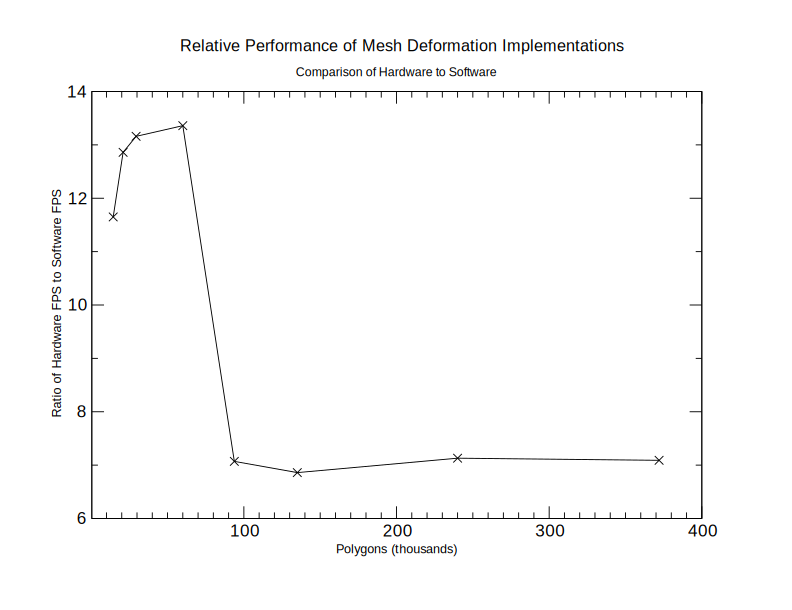
\includegraphics[width=0.9\textwidth]{performance}
\caption{\label{fig:performance}A plot of the ratio between FPS using the
GPU-based implementation and the pure-software implementation.}
\end{figure}

To test the relative performance of software and hardware two implementations
were made, one software and one hardware. Both implemented the same mesh deformation
algorithm as above and both used as near equal, within the intersection of C and
Cg, implementations of the generator exponentiation and rotor application
routines.

The implementations differed most in the use of display lists. To mirror real-world
practises each model in the hardware implementation was uploaded to the graphics
card in a display list since the per-vertex set of $d_{k,i}$ and $p_i$ could
be pre-computed. In the software implementation these were also pre-computed but the
deformed vertices had to be uploaded to the graphics card once-per frame since the
deformation step was done in software.

Table \ref{tab:performance} shows the number of frames per second that could be
displayed with a simple cube model at various different polygon count. A simple model
was chosen so that the generation, per frame, of un-deformed model vertices in the
software implementation would take as little time as possible being 
algorithmically generated rather than fetched from main memory providing a fairer
test of the speeds of the deformation algorithm. Figure \ref{fig:performance} shows
the ratio of improvement between software and hardware implementations with polygon
count.

\section{Dynamics}

In this section we will develop a simple method for doing dynamics with a sphere
which has been deformed with a set of rotors. We shall show how a simple dynamics example
using such a method may be implemented on the GPU.

Recall that a GPU has two classes of shaders; it has vertex shaders which are applied
per-vertex and fragment shaders which are applied per-pixel. Since, in a typical scene,
one would expect the number of pixels on screen to be very much greater than the number
of vertices, GPUs generally have more parallel fragment shaders than vertex shaders.
If we can re-formulate our solution to use fragment shaders we might expect even
greater performance than simply using the vertex shader.

Algorithms implemented on the fragment shaders have one further 
advantage when compared to those implemented on the vertex shader when one makes use
of the \emph{render to texture} feature on modern graphics cards. Using this feature
rendering can be directed to a texture stored in the graphics card memory rather than the
screen. This feature allows iterative algorithms to be developed.
The concept is simple. A texture is created which stores a set of initial values. 
A square is then rendered with a fragment shader which, for each pixel in the square,
reads the initial value from the texture and outputs the result of the next iteration.
If this square is rendered into the original texture then the result of each iteration
replaces the previous one. This process may be repeated as often as is desired.
In reality there are a few implementation issues. Aside from the API calls required to
setup the render to texture and appropriate projection matrices a significan issue is
that the shader is required to write back to its input which could lead to
concurrency issues. To avoid this one generally uses two textures, an `input' and `output',
which are swapped between each iteration.

\subsection{Collision detection via deformation}

\begin{figure}
\centering
\includegraphics[width=0.8\textwidth]{deformation_scheme}
\caption{\label{fig:deformation_scheme}Given a deformation scheme $\mathcal{D}$ which maps
  our object to the unit sphere we can tell whether a point, $P$, is inside the object by
          testing if the mapped point, $P'$, is inside the sphere.}
\end{figure}

We shall develop a simple example to illustrate this method. In our example we shall 
implement an approximate simulation of a cloth falling onto a complex smooth object.
Our approach is illustrated in figure \ref{fig:deformation_scheme}. We shall assume
some GA-based deformation scheme $\mathcal{D}$ which will deform our object to the
unit sphere. Ideally this deformation scheme should preserve both position and orientation
information so that we can perform physics on the unit sphere and deform the result back to 
our original object.

\begin{figure}[p]
\centering
\scalebox{0.7}{
\begin{minipage}{\textwidth}
\singlespacing
\lstinputlisting[language=c]{map.cg}
\end{minipage}}
\caption{\label{fig:map}The vertex shader utility functions for mapping to and
  from a rotor-deformed space.}
\end{figure}


\chapter{Conclusions and Future Work}

In this chapter we shall collate all of the findings from the previous chapters
and give them a context in relation to each other. Future applications for
the various findings will also be discussed.

\section{Review of Achievements}

In this section we briefly review the achievements and findings from each
chapter.

\subsection{Non-Euclidean geometries}

In chapter \ref{chap:noneuclid}, a framework for extending the conformal
model to deal with non-Euclidean geometries was developed, with particular
emphasis on hyperbolic geometry. It was shown that the geometry
represented by a model is entirely determined by the choice of null-vector
representation and rotors. The pure-rotation and pure-translation 
rotors for hyperbolic space were derived and it was shown that from them the usual
distance metric for hyperbolic geometry could be obtained.

Already some work using the conformal model to represent non-Euclidean geometry
has found application in cosmology\cite{GA:SIGKEY} has been done leading, potentially, to important insights on
our universe.

\subsection{Fractals}

In chapter \ref{chap:fractals} an extension to complex numbers, similar to that
of quaternions, was developed for arbitrary dimension. It was noted that, in
GA, quaternions are simply special cases of a wider variety of algebras. This
extension was used to form a dimension-agnostic formulation for the classic
complex iteration-based Julia and Mandelbrot fractal sets. In addition an
existing distance estimation formula was shown to be valid using this extension
allowing for the ray-tracing of arbitrary dimension sets.

Real-world applications of fractals are notoriously difficult to find but the
opening up of escape-time fractals to non-Euclidean geometries provides a
number of opportunities for `recreational mathematics' and the generation of
attractive images.

\subsection{Rotor exponentiation}

In chapter \ref{chap:exponential} it was hypothesised that all the rotors we
used in the conformal model could be obtained by exponentiating a corresponding
generator bivector the components of which would be geometrically meaningful.
A closed form solution for \emph{both} the exponentiation and subsequent
inverse exponentiation (modulo the identification of rotations by $2n\pi$) was
derived.

From this an algorithm for directly mapping the components of the generator
to a $4 \times 4$ matrix suitable for use in existing graphical pipelines
was developed. A matching algorithm for directly converting a matrix to
a generator, again identifying rotations of $2n\pi$, was also developed.

This particular chapter has almost limitless application. Not only is the
linear space of the bivectors mapped to the non-linear space of rigid-body
transformations but the appropriate inverse mapping was also defined. Using
this method many existing linear optimisation algorithms or interpolation
schemes could be extended to deal with rotation and translation
\emph{simultaneously}.

\subsection{GPU-based techniques}

In chapter \ref{chap:gpu} the techniques developed in chapter \ref{chap:exponential}
were implemented on the programmable portion of modern Graphics Processing
Units. Such \emph{shaders} were used to develop sample graphics algorithms which
made use of the mappings developed in this thesis. 

Specifically simple mesh deformation and collision detection examples were show.
The examples demonstrated that not only was GA a natural language for developing
such algorithms allowing one to use much geometric insight but they were also
compact enough to program so that they could be efficiently implemented in hardware.

\section{Future work}



\end{mainmatter}

% \nocite{*}

\begin{backmatter}
\bibliography{header,bibliography,geometry,ga,fractals,fractal_coding}
\end{backmatter}

\end{document}
